\chapter{Modellentwurf}\label{sec:modellentwurf}
Nachdem nun alle notwendigen Grundlagen erläutert wurden, wird in diesem Kapitel der Grid Fin samt Aktuatorik entworfen. Hierzu werden zunächst die Anforderungen an das System aufgestellt, um dann auf dieser Basis eine geeignete Wahl der Designvarianten treffen zu können. Zur Übersicht über die verschiedenen technischen Umsetzungsvarianten wird ein morphologischer Kasten zur Hilfe gezogen. Des Weiteren wird in diesem Kapitel die erste Version des Grid Fins in CAD modelliert.
\section{Systemanforderungen}
Zunächst werden also die Anforderungen an das System definiert. Hierbei wird sich hauptsächlich auf eine in Matlab mit Simulink durchgeführte Simulation des gesamten Missionsablauf der Valkyrie und Angaben von GAIA Aerospace bezogen.
\subsection{Anforderungen an die Aerodynamik}
Das Wichtigste ist natürlich, dass die Grid Fins ihre Funktion erfüllen, beim Wiedereintritt einen stabilen Flug zu gewährleisten. Simulationen haben ergeben, dass hierfür ein Beiwertanstieg von $C_{N\alpha} =0,048/^\circ=2,75/$rad und einer Fläche $A=0,09\mathrm{m}^2$ erforderlich sind. Die zu entwerfenden Finnen sollten also vergleichbare Normalkräfte produzieren können.

Auch wenn die Axialkraft zusätzlich zur Stabilität beiträgt, ist sie weniger wichtig und liegt in den bisherigen Simulationen bei $C_X=0,1$ für $\mathrm{Ma}_\infty=2.0$ bei einem Anstellwinkel von $0^\circ$. Auch wenn ein größerer aerodynamischer Widerstand den Vorteil hat die Triebwerke, beim Bremsen zu entlasten, sollte dies jedoch nicht auf Kosten der Lebensdauer der Grid Fins passieren, weil sonst der Aspekt der Wiederverwendbarkeit eingeschränkt wird. Mehr Widerstand würde des Weiteren eine geringe Gleitzahl zur Folge habe. Da die Grid Fins eventuell dafür genutzt werden sollen dem Auffanghelikopter entgegen zu gleiten, wäre eine möglichst großes Auftrieb-zu-Widerstand-Verhältnis wünschenswert. Außerdem schadet ein hoher Widerstand der Wirtschaftlichkeit, weil die höheren Kräfte stärke Belastungen verursachen würden, was wiederum hohere Masse und Kosten der Lagerung und Aktuatoren zur Folge hat.
\subsection{Leistungsanforderungen}
Die Aktuatoren müssen nun gewährleisten, dass die Grid Fins zu jedem Zeitpunkt unter gegebener Last die notwendige Position einnehmen können. Für den Klappwinkel sind die Anforderungen an den Motor und das zugehörige Getriebe also sehr gering. Die Bewegung passiert hier ohne angreifende Kräfte, sodass nur die eigene Trägheit und die Lagerreibung überwunden werden muss. Dabei ist auch keine hohe Drehrate erforderlich, da für dieses Manöver theoretisch der gesamte Zeitraum zwischen Separation und Wiedereintritt zur Verfügung steht. Danach muss nur noch dafür gesorgt werden, dass die Grid Fins diese Position halten. Die größte Belastung tritt für die Klappwinkelaktuatorik dann auf, wenn der Ballonschirm ausgelöst wird und die Grid Fins an ihrer Einspannung ruckartig herum gerissen werden, was ein unerwünschtes Moment bewirkt. Die aerodynamische Axialkraft wirkt hier zwar helfend entgegen, liegt jedoch eine ganze Größenordnung unter den Trägheitskräften.
Der Klappwinkel muss also einmal von $\Lambda=90^\circ$ zu $\Lambda=0^\circ$ bewegbar sein und sich dort halten lassen.
\\~\\
Der Aktuator für das Steuergelenk aber muss deutlich höhere Leistungen aufbringen können. Der Steuerwinkel wird während des Wiedereintritts ständig vom Regler verändert, um die gewünschte Orientierung zu erhalten. Somit kommen zu den Trägheits- und Reibungskräften auch noch das aerodynamische Moment, bzw. Steuermoment, hinzu. Wenn auch deutlich größer als die auftretenden Momente beim Klappwinkel, sind sie dennoch im Vergleich zu planaren Finnen noch immer gering, wie in dem vorherigen Kapitel gezeigt wurde. Im Gegensatz zum Klappwinkel spielt hier auch die Drehrate eine wichtige Rolle, da nur wenn die Grid Fins auch schnell genug reagieren, der Flug effizient geregelt werden kann. In der Simulink-Simulation kommt es bei unbeweglichen Grid Fins zu Schwingungen in der aerodynamischen Flugphase mit einer Periodendauern von $\Delta t=0,73$s unter Extrembedingung, wie in Abschnitt \ref{sec:MechAnford} noch zu sehen sein wird. Um diese auszugleichen, muss also auch der Steuerwinkel in der gleichen Zeit aus der Ruhelage ($\delta = 0^\circ$) zum maximalen Ausschlag in die eine Richtung ($\delta = 20^\circ$), dann in die andere ($\delta = -20^\circ$) und wieder zurück bewegt werden.
\subsection{Anforderungen an die Kosten}
Für die Kosten gilt das klare Ziel diese zu minimieren und somit maximale Wirtschaftlichkeit zu erreichen. Somit sollen, so weit es geht, COTS verwendet werden, die keine teure Sonderanfertigung benötigen. Es gilt auch möglichst kleine und leichte Bauteile zu verwenden, dadurch kann doppelt eingespart werden, da zum einen weniger Materialkosten entstehen und zum anderen auf Grund des geringeren Gewichts der Treibstoffverbrauch reduziert und mehr Nutzlast transportiert werden kann.
\subsection{Thermische und mechanische Anforderungen}\label{sec:MechAnford}
Beim Wiedereintritt treten sehr hohe thermische Lasten auf, die sich jedoch schwer im Vorfeld quantifizieren lassen, da sie stark von der Geometrie abhängen und sich nur durch aufwendige CFD-Simulationen bestimmen lassen. Generell gilt für die thermische Belastung, dass umströmte Fläche, besonders an der Vorderkante, einen negativen Effekt hat und die Wärme des durch den Verdichtungsstoß stark erhitzen Fluids aufnimmt. Währenddessen ist ein großes Volumen mit idealer Weise hoher Wärmekapazität vorteilhaft, da dieses die Energie der Außenfläche aufnehmen kann. Dieser Effekt ist am besten bei hoher Wärmeleitfähigkeit nutzbar und sorgt für möglichst geringe Temperaturgradienten, die wiederum auch Eigenspannungen verursachen würden. Am wichtigsten ist jedoch die Schmelztemperatur beziehungsweise die maximale Temperatur, bei der der Werkstoff noch akzeptable mechanische Eigenschaften hat, weil dies schlussendlich bestimmt, wie viel Wärme ausgehalten werden kann.
\\~\\
Für die Stabilität gilt, dass sich die Grid Fins und natürlich auch ihre Aktuatorik nicht plastisches verformen oder gar vollständig versagen dürfen. Dabei ist auch besonders auf das Kriechen zu achten, welches bei einer Kombination von thermischer und mechanischer Belastung, wie sie hier vorliegt, schnell auftreten kann.

Abbildung \ref{abb_KraefteNormal} zeigt die für alle vier Grid Fins gleich angreifenden Kräfte im körperfesten System bei einer Mission der Valkyrie, wenn sie durchgehend in der Neutralstellung gehalten und nicht gesteuert oder geregelt werden. Dargestellt sind sowohl die Kräfte in $X_b$-Richtung (rot), als auch in $Y_b$- (blau) und $Z_b$-Richtung (grün) im Zeitintervall von $t=400$s bis $t=500$s nach der Entkoppelung vom Pylon. Während die Axialkraft relativ monoton steigt und fällt, sind die Normalkräfte starken Schwankungen auf Grund der Abwesenheit eines Reglers ausgesetzt.

Es ist zu erkennen, dass bei ungefähr $t=400$s mit einer Machzahl von $Ma \approx 8.0$ bei einer von Höhe 66,5km  der Wiedereintritt beginnt und die Kräfte anfangen zu steigen. Diese schwellen schnell auf und der Lastenvektor $\vec{F}$ erreicht seinen Höhepunkt bei
\begin{equation}
	\vec{F}(t=448,5\mathrm{s})=
		\left(\begin{array}{c}F_{x}\\F_y\\F_z\end{array}\right)
			=\left(\begin{array}{r}487\mathrm{\ N}\\70\mathrm{\ N}\\220\mathrm{\ N}\end{array}\right).
\end{equation}
An dieser Stelle ist der maximale Staudruck "Max Q"\ bei einer Machzahl von $Ma = 3.7$ auf einer Höhe von 20km erreicht und wird für die Auslegung von entscheidender Bedeutung sein. Danach nehmen alle Kräfte wieder ab, da sich die Geschwindigkeit verlangsamt. 
\begin{figure}[h]
	\centering
	\includegraphics[width=0.9\textwidth]{FNormal.png}
	\caption{Kräfte an den Grid Fins bei konstant gehaltener Neutralstellung}
	\label{abb_KraefteNormal}
\end{figure}\\
Dies kommt dadurch zustande, dass die Dichte der Umgebungsluft zwar monoton steigt, die Geschwindigkeit aber abnimmt. Diese ist in Abbildung \ref{abb_vNormal} für den selben Zeitbereich dargestellt. Am Anfang macht sich die Atmosphäre noch nicht stark bemerkbar, dort steigt sogar die Geschwindigkeit durch die Flugbahn leicht an. Es folgt der ReEntry-Burn, der die Rakete von $\vec{U}_\infty \approx 2.500$m/s auf etwas über $1.500$m/s abbremst. Danach lässt sich der Widerstand in der Atmosphäre an dem weiteren Abfallen der Fluggeschwindigkeit erkennen, deren Zeit mit den Kräften in Abbildung \ref{abb_KraefteNormal} übereinstimmt. Diese Reduzierung der Geschwindigkeit erklärt die Abnahme der aerodynamischen Kräfte an den Grid Fins. Bei ungefähr $t=456$s ist ein Knick in der Geschwindigkeitskurve zu erkennen, der den Zeitpunkt markiert, an dem eine Machzahl von 2 unterschritten wird, sodass der Ballute auslöst. Dies mindert die Geschwindigkeit weiter drastisch ab, damit sich der Gleitschirm sicher öffnen kann. Der Zeitraum nach dem Öffnen des Ballonschirm ist für die Auslegung der Grid Fins uninteressant.
\begin{figure}[h]
	\centering
	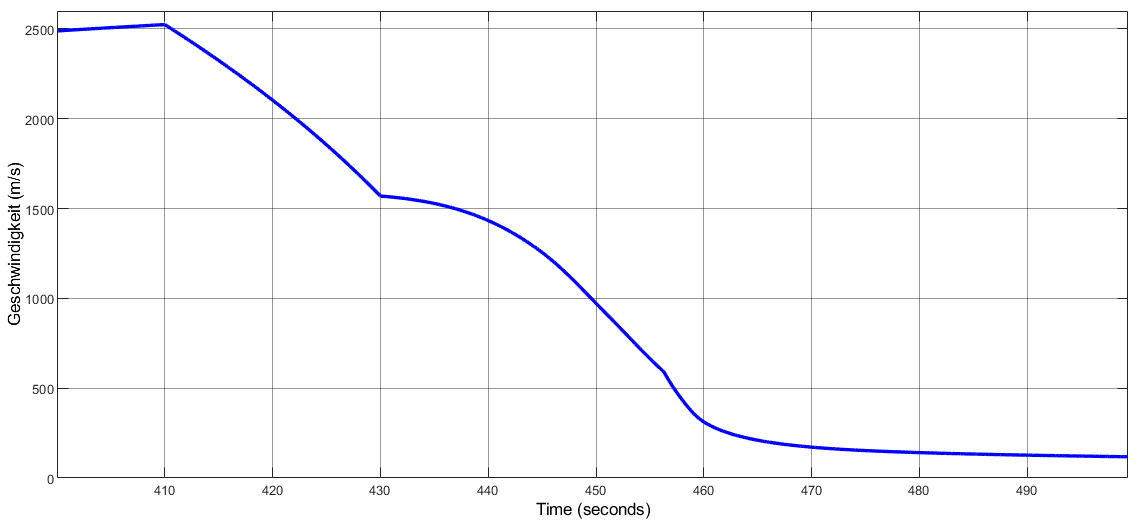
\includegraphics[width=0.9\textwidth]{vNormal.png}
	\caption{Fluggeschwindigkeit bei konstant gehaltener Neutralstellung}
	\label{abb_vNormal}
\end{figure}\\~\\
Dies war nun aber nur ein standardmäßiger Missionsablauf, der den Grid Fins nicht viel abverlangt. Für die Auslegung müssen jedoch auch die Worst-Case-Szenarien berücksichtigt werden. Dazu zählt zum einem ein Ausschlag des Steuerwinkels, wodurch zum einem deutlich höhere Normalkräfte zu Stande kommen, aber auch die Axialkräfte deutlich ansteigen. Des Weiteren ist der Fall zu betrachten, dass der ReEntry-Burn ausfällt, beziehungsweise bewusst weggelassen wird, um die Wirtschaftlichkeit durch geringere Treibstoffmitnahme zu maximieren. In dem Fall würde die Raketenstufe mit deutlich höherer Geschwindigkeit in die Atmosphäre eintauchen, was zu enormen Belastungen führt.

Zu dem maximalen Lastfall kommt es, wenn kein ReEntry-Burn stattfindet und alle Grid Fins um $\delta = \pm 10^\circ$ ausgeschlagen sind. Die Finnen befinden sich dabei in x-Formation und der Ausschlag ist so ausgerichtet, dass ein Moment erzeugt wird, das den Nickwinkel verringert. Die Kräfte im körperfesten Koordinatensystem, die in diesem Fall von den Grid Fins ausgehalten werden müssen, sind für die gegenüberliegenden identisch. Abbildung \ref{abb_FExtreme} zeigt die Kräfte an einem der Grid Fins. Während der Widerstand nur leicht ansteigt, nehmen die Normalkräfte sehr hohe Werte an, wie der Kraftvektor
\begin{equation}
	\vec{F}_b(t=440,7\mathrm{s})
	=\left(\begin{array}{r}817\mathrm{\ N}\\-6.530\mathrm{\ N}\\-6.183\mathrm{\ N}\end{array}\right)
\end{equation}
zeigt. Um den nun wirklich am Grid Fin angreifenden Lastfall zu erhalten, müssen diese Kräfte noch entsprechend transformiert werden. Zu erkennen ist außerdem, dass der Wiedereintritt hochfrequenten Schwingungen auslöst, die Amplituden von bis zu $\Delta F_z = 3.194$N besitzen. Wird nun aber davon ausgegangen, dass eine funktionstüchtige Regelung existiert, so kann diese Schwingung ausgeglichen werden und es käme ein Kraftvektor mit den folgenden Mittelwerten zu Stande:
\begin{equation}\label{eq_Fmax}
\vec{F}_\mathrm{b, 1, geregelt}(t=440,7\mathrm{s})
=\left(\begin{array}{r}572\mathrm{\ N}\\-6.415\mathrm{\ N}\\-4.995\mathrm{\ N}\end{array}\right)
\end{equation}
\begin{equation}\label{eq_Fmax2}
\vec{F}_\mathrm{b, 2, geregelt}(t=440,7\mathrm{s})
=\left(\begin{array}{r}568\mathrm{\ N}\\6.415\mathrm{\ N}\\-5.030\mathrm{\ N}\end{array}\right)
\end{equation}
Die 1 steht dabei für die Kräfte an den Grid Fins D1 und R2 und die 2 für R1 und D2.
Der Moment, in dem eine Machzahl von $Ma_\infty = 2$ erreicht wird und der Ballonschirm auslöst, ist zwar auch in Abbildung \ref{abb_FExtreme} deutlich erkennbar, da die Raketenstufe in zu diesem Zeitpunkt plötzlich herumgerissen wird, kann jedoch im Vergleich zu den Kräften bei "Max Q"\ vernachlässigt werden.
\begin{figure}[h] 
	\centering
	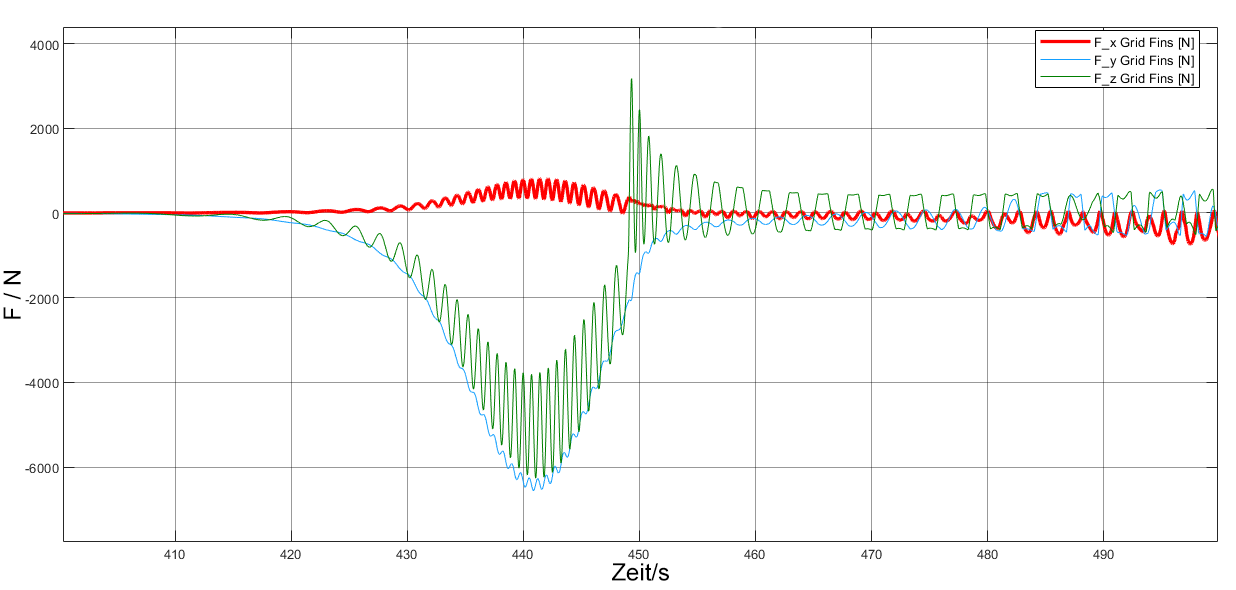
\includegraphics[width=0.8\textwidth]{F2Extreme4.png}
	\caption{Kräfte am Grid Fin R1 beim maximalen Lastfall}
	\label{abb_FExtreme}
\end{figure}
\begin{figure}[h] 
\centering
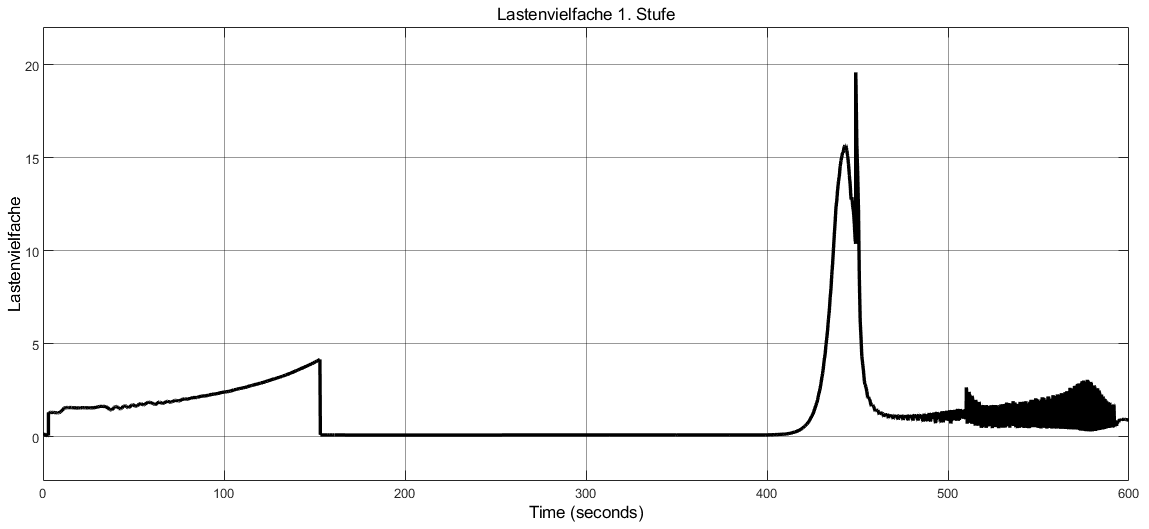
\includegraphics[width=0.8\textwidth]{n_x.png}
\caption{Lastvielfache der ersten Stufe in x-Richtung über gesamten Missionsverlauf beim maximalen Lastfall}
\label{abb_n_x}
\end{figure}\\
Was nicht zu vernachlässigen ist, sind die Trägheitskräfte, die dabei entstehen. Die Grid Fins werden an ihrer Einspannung schlagartig, wenn auch nur kurzzeitig, belastet. Abbildung \ref{abb_n_x} zeigt, dass, auch wenn schon beim ReEntry-Burn und durch den aerodynamischen Widerstand hohe Lastvielfache auftreten, die Beschleunigung von fast 20$|\vec{g}|$ bei der Abbremsung durch den Ballonschirm der kritischste Moment in Hinblick auf die Trägheitskraft ist.
\subsection{Geometrische Anforderungen}
Die Hauptmaße der Grid Fins sind hauptsächlich durch die Fertigung begrenzt. Ein Grid Fin soll also in einen entsprechenden 3D-Drucker mit den Maßen $300$x$300$x$400\mathrm{\ mm}^3$ passen. Für die Größe und Anordnung der Aktuatorik ist darauf zu achten, dass für alle vier Grid Fins jeweils zwei Motoren mit ihren zugehörigen Getrieben in den Raketendurchmesser von $1,10$ m passen müssen. Es ist des Weiteren eine Maximalhöhe von $0,15$ m vorgesehen, die nicht überschritten werden darf. Dieser Raum darf aber auch nicht vollständig gefüllt werden, da die Bordelektronik in diesem Bereich auch Platz finden muss.
\section{Morphologische Kästen}
Um eine Übersicht über die verschiedenen Designmöglichkeiten zu haben, werden an dieser Stelle zwei morphologische Kästen, jeweils einen für das Design des Grid Fins und die Gestaltungsmöglichkeiten der Aktuatorik, eingeführt. Für fünf Designentscheidungen des Grid Fins sind hier unterschiedliche Teillösungen aufgelistet.
\subsection{Morphologischer Kasten des Grid Fins}
\begin{figure}[h]
	\centering
	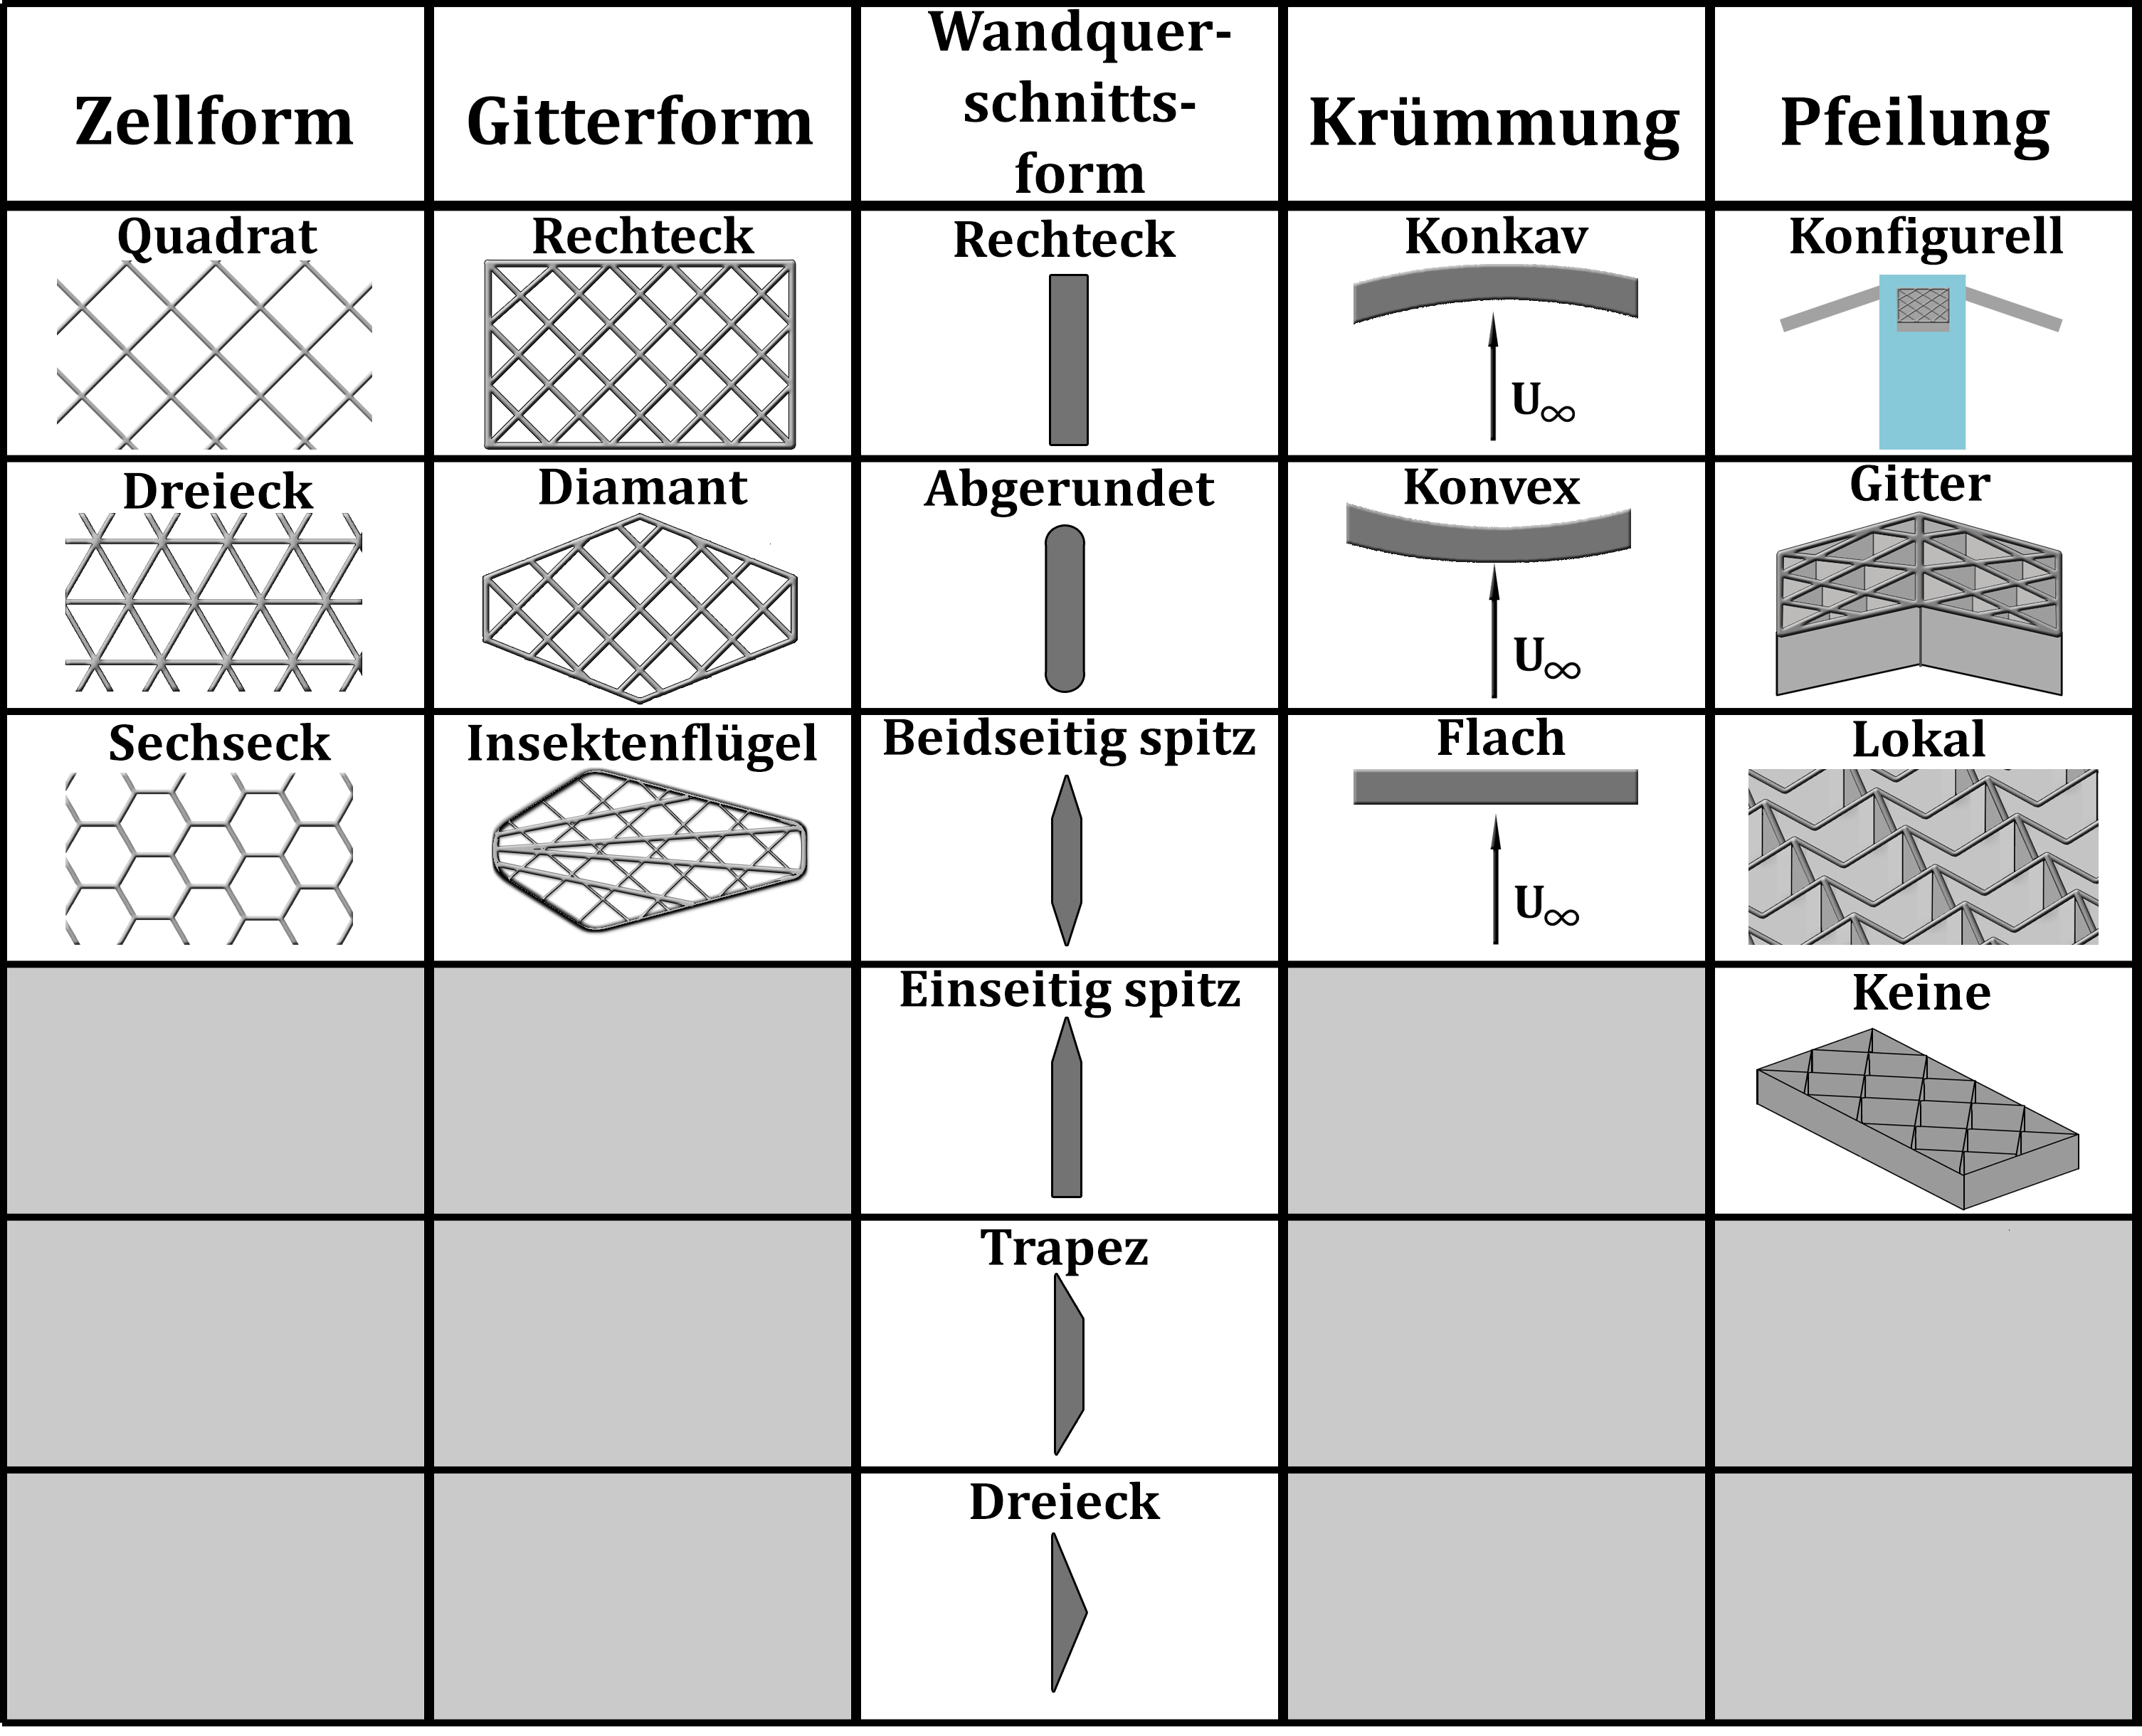
\includegraphics[width=0.9\textwidth]{Morphologischer Kasten GF V2.png}
	\caption{Morphologischer Kasten für die Grid Fins}
	\label{abb_MorphKastGF}
\end{figure}
Ganz links sind drei mögliche Zellformen gegeben. Es besteht die Wahl zwischen quadratischen, drei- und sechseckigen Geometrien. Hierbei sei aber wieder zu berücksichtigen, dass es auch zu einer Mischung mehrerer Formen kommen kann und besonders am Rand durch den Rahmen die Zellen ungleichmäßig verkleinert werden können.

Für die Form des gesamten Gitters stehen auch drei unterschiedliche Optionen zur Auswahl: Rechteck, Diamant oder auch eine dem Insektenflügel nachempfundene Struktur. Da jedoch die Maße noch nicht festgelegt sind, kann die ersten der beiden Formen auch noch zum Quadrat werden. Des Weiteren kann es sein, dass die Geometrie an der einen Seite für die Anbringung noch angepasst wird.

Die größte Auswahl bietet sich bei den Wandquerschnittsformen. Rechteckig, abgerundet, beidseitig und einseitig spitzt, trapezförmig und dreieckig sind die sechs Optionen, die es hier gibt. Der Wandquerschnitt muss nicht überall die gleiche Form besitzen. So kann es sein, dass das Gitter eine andere Form erhält als der Rahmen. Die unteren beiden Formen sind zum Beispiel asymmetrisch, sodass sie nur für die Umrandung der Grid Fins in Frage kommen.

Als viertes wird die Fragestellung einer Krümmung gezeigt. Neben einem flachen Design kann der Grid Fin entweder zur Strömung hin konvex oder konkav gekrümmt sein. Dies ist von Bedeutung, wenn der Grid Fin in die eine oder andere Richtung geklappt und an den Körper angelegt werden soll.

Im Grundlagenkapitel wurden drei verschiedene Arten der Pfeilung eines Grid Fins gezeigt. Da sie sich grundsätzlich unterschiedlich implementieren lassen, können sie theoretisch sogar in Kombination gewählt werden. Der Pfeilungswinkel ist für die Varianten noch frei wählbar und auch negative Winkel, also Vorwärtspfeilung, ist denkbar. Für die lokale Pfeilung ist eine Unterscheidung zwischen Vorwärts- und Rückwärtspfeilung nicht sinnvoll, stattdessen gibt es hier aber den Berg- und Tal-Typus. Wichtig ist noch anzumerken, dass die konfigurelle Pfeilung keinen direkten Einfluss auf das Design der Grid Fins an sich hat, sondern sich durch den Bewegungsspielraum der Aktuatorik umsetzten lässt.\\
Es gibt jedoch noch weitere Designentscheidungen, die sich nicht in einem morphologischen Kasten pragmatisch darstellen lassen. So müssen zum einen noch die Dimensionen des Moduls und Lage der Aktuatoren in der Rakete definiert werden. Zum anderen stellt sich die Frage, welche Zellgröße $g$ und Wandstärke $d$ an welcher Stelle gewählt wird. Es besteht auch noch die Möglichkeit die Grid Fins mit zusätzlichen Features auszustatten. Eine Option wären hier zusätzliche Stützstreben oder sogar durch die additive Fertigung ermöglichte, in das Material integrierte Strukturen, wie zum Beispiel Kühlkanäle oder Drucksensoren.
\subsection{Morphologischer Kasten der Aktuatorik}
Für den Entwurf der Aktuatorik wird ein zweiter morphologischer Kasten zur Hilfe genommen. Dieser ist in Abbildung \ref{abb_MorphKastAk} zu sehen und zeigt drei verschieden Designkategorien. Da die Grid Fins zwei unabhängige Freiheitsgrade haben, können für den Steuer- und Klappwinkel separat unterschiedliche Lösungen aus dem morphologischen Kasten gewählt werden.
\begin{figure}[h]
	\centering
	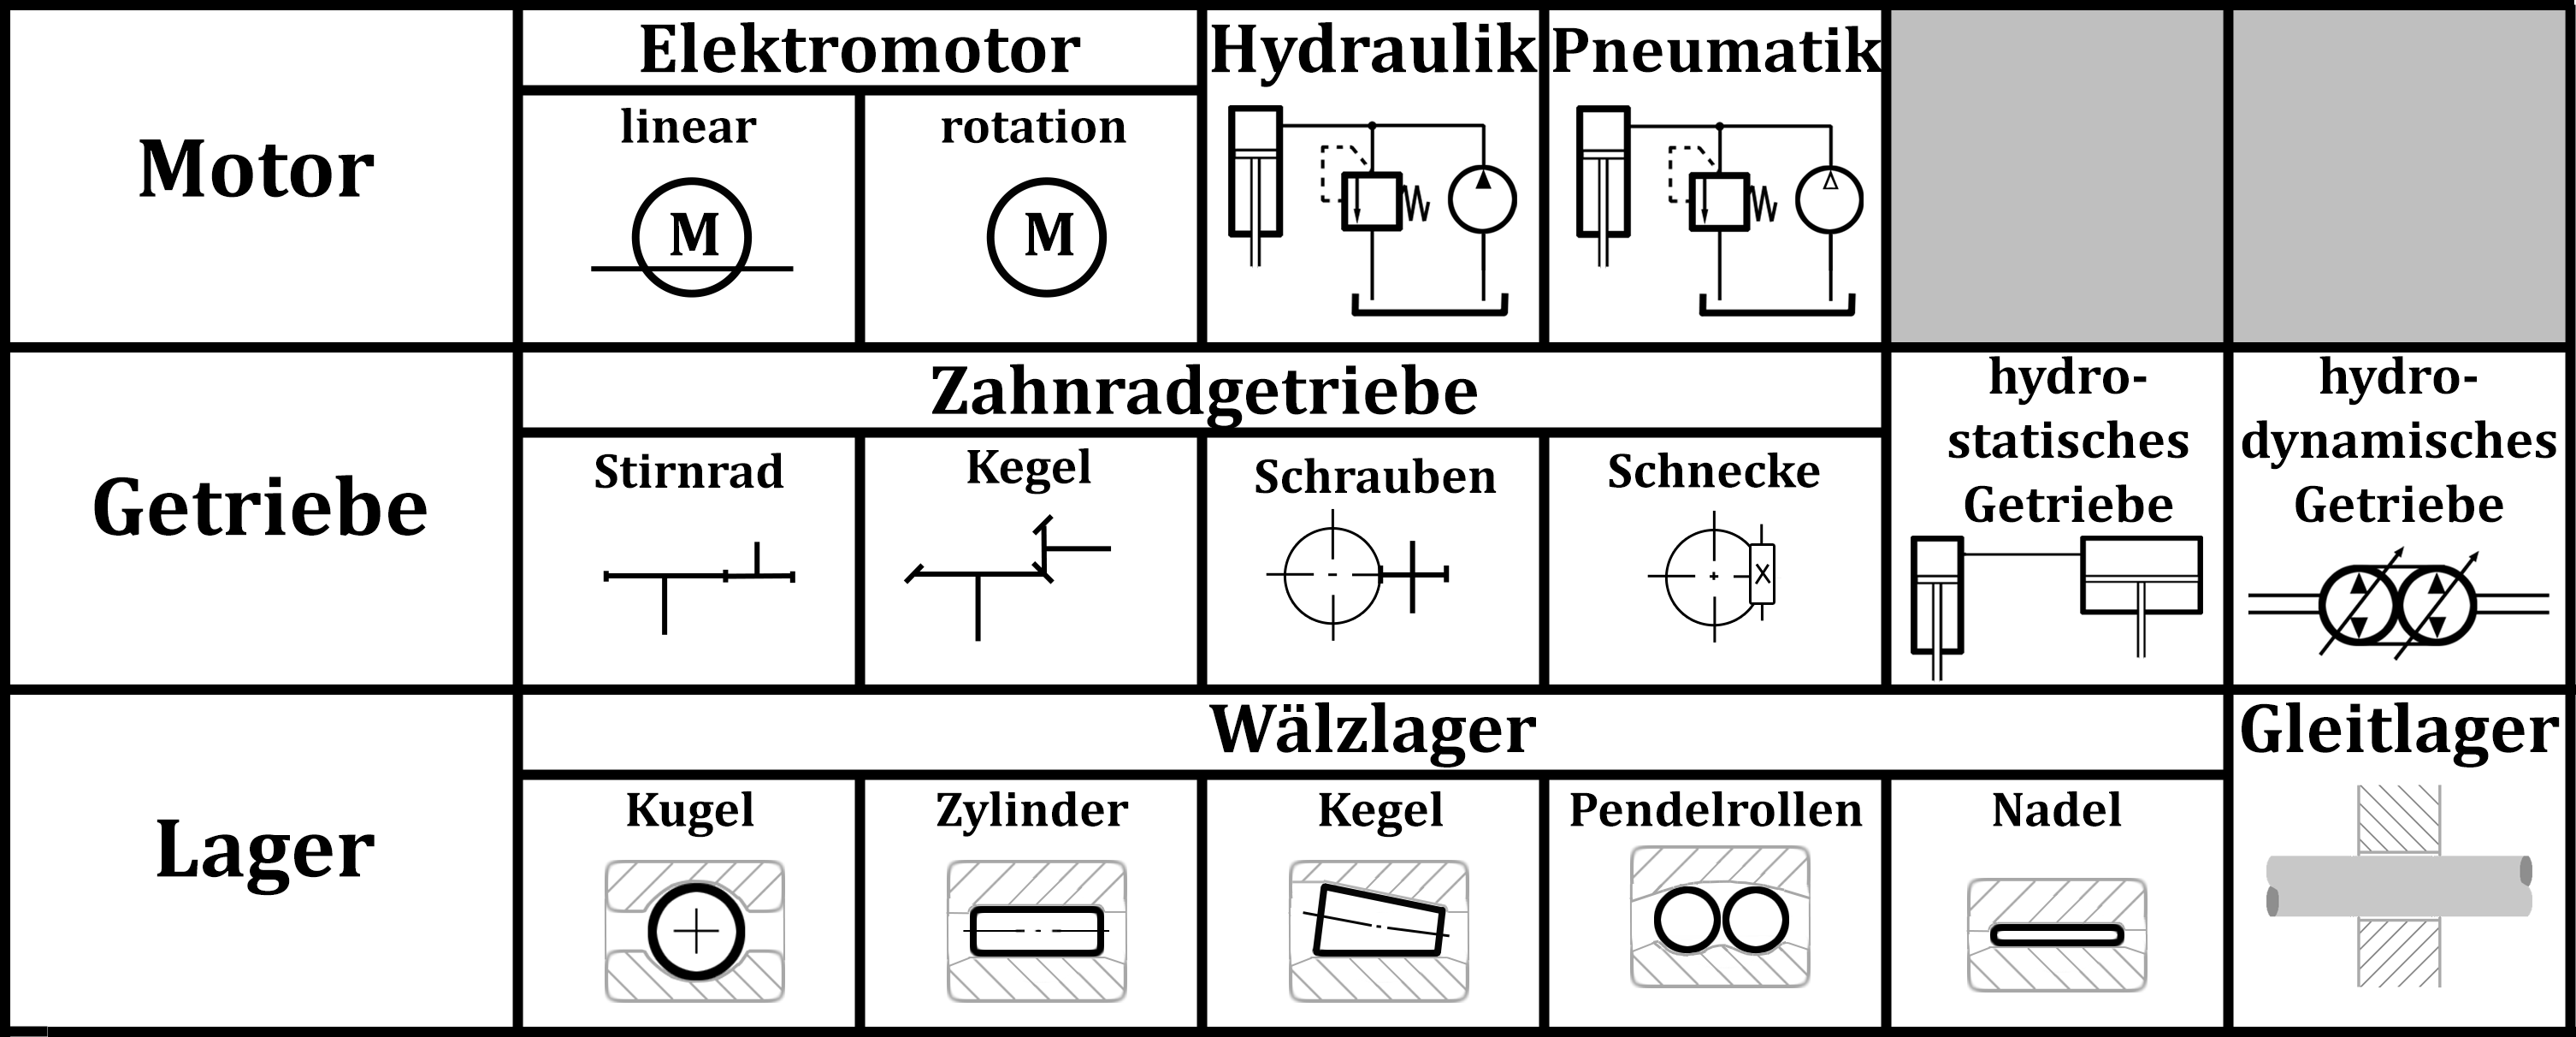
\includegraphics[width=\textwidth]{Morphologischer Kasten Ak.png}
	\caption{Morphologischer Kasten für die Grid Fin Aktuatorik}
	\label{abb_MorphKastAk}
\end{figure}\\
Eine wichtige Designentscheidung ist der Aktuator, da er bestimmt, was als Energiequelle genutzt wird, und hat somit einen großen Einfluss auf Gewicht und Kosten. Eine Möglichkeit ist die elektrische Energie zu nutzen und diese mit einem Elektromotor direkt die mechanische Arbeit verrichten zu lassen. Hierbei muss noch die Wahl getroffen werden, ein linearer oder rotatorischer Motor vorgezogen werden soll. Alternativ kann auch ein hydraulisches oder gar pneumatisches System verwendet werden. Da Grid Fins zwei Freiheitsgrade haben, können diese über unterschiedliche Aktuatoren, die auch unterschiedlicher Art sein können, bewegt werden. Also muss in diesem Punkt für beide Rotationen einzeln entschieden werden.

Über ein Getriebe wird die Leistung des Aktuators auf die Grid Fins übertragen, um mehr Spielraum für Kraft, Moment, Drehzahl und Orientierung des Aktuators zu gewährleisten. Eine Möglichkeit bietet das klassische Zahnradgetriebe. Viele Paarungen wie Stirn-, Kegel-, Schrauben- oder Schneckenräder sind denkbar. Kräfte und die zugehörige Bewegungsgeschwindigkeit lassen sich auch durch hydrostatische Getriebe beeinflussen. Momente und Drehzahlen können durch hydrodynamische Getriebe verändert werden. Generell sind durch Kombinationen beliebig komplexe Systeme möglich.

Als letztes beschäftigt sich der morphologische Kasten in Abbildung \ref{abb_MorphKastAk} mit der Lagerung. Hierbei wird generell zwischen den Wälz- und Gleitlagern unterschieden. Beide bieten jedoch noch mehr Entscheidungsfreiheiten. So gibt es einige unterschiedliche Wälzkörper wie Kugeln, Zylinder, Kegel oder Pendelrollen. Auch Gleitlagern können weiter zu statischen und dynamischen unterteilt werden, je nach Art der Schmierfilmdruckerzeugung.
\section{Modellierung des Grid Fins}
Nun kann mit Hilfe des morphologischen Kastens der Grid Fin modelliert werden, sodass alle Anforderungen bestmöglich erfüllt werden. Bevor jedoch die Designoptionen aus Abbildung \ref{abb_MorphKastGF} gegeneinander abgewogen werden, wird das Material, aus den der Grid Fin gefertigt werden soll, bestimmt. Danach werden die einzelnen Parameter festgelegt, um eine anschließende Implementierung in CAD zu ermöglichen.
\subsection{Materialwahl}
Es stehen vier verschiedene Werkstoffe zur Auswahl, die sowohl für die Raumfahrt, als auch additive Fertigung in Frage kommen: Edelstahl, Nickel- (Inconel), Aluminium- und Titanlegierungen. Tabelle \ref{tab_Werkstoffe} im Anhang zeigt Vertreter dieser Werkstoffgruppen, wie sie vom 3D-Druck-Anbieter EOS benutzt werden, und vergleicht ihre Eigenschaften. Die vielversprechendsten Vertreter der jeweiligen Werkstoffgruppen, oder jede zu denen genügend Daten vorliegen, sind zusätzlich der Übersicht halber ein weiteres Mal in Tabelle \ref{tab_WerkstoffeKlein} dargestellt.
\begin{table}[h] 
	\centering 
	\caption{Vergleichsdaten der unterschiedlichen Werkstoffe (Auswahl) \\ (Preise in Bezug auf ein 100 mm$^3$ Modell, vgl. Abbildung \ref{abb_100mmModel})}
	\label{tab_WerkstoffeKlein}
	\begin{tabular}{c|c|c|c|c|c|c|c} 
		Werkstoff&Bezeichnung&$\rho$/$\frac{k\mathrm{g}}{\mathrm{cm}^3}$&$R_{p,0.2}$/MPa&$R_\mathrm{spez.}$/Nm/g&Preis/€&$T_\mathrm{E, max}$/$^\circ$C&$T_\mathrm{Schmelz}$/$^\circ$C\\ 
		\hline 
		Aluminium&AlSi10Mg&2,57&230-270&89,5&1.508,93&530&557\\ 
		Edelstahl&1.4542&7,79&861-861&110,5&2.559,27&550&1400\\ 
		Inconel&IN 718&8,15&1140-1245&140,5&2.597,71&700&1260\\ 
		Titan&TiAl6V4&4,41&1120-1140&254,0&3.085,12&>700&1630\\ 
	\end{tabular} 
	\begin{flushright} 
		\flushbottom{Quellen: \cite{eos, preise, T1.1, T1.4, T2.1, T2.4, T2.3, T3.5, T3.8}} 
	\end{flushright} 
\end{table} \\
Eine wichtige Eigenschaft ist natürlich die Dichte $\rho$. Hier liegen die Aluminiumlegierungen ganz klar vorne mit nur $2,57$ g/cm$^3$, aber auch Titan bietet vergleichsweise gute Werte. Die Edelstähle und Nickellegierungen hingegen sind deutlich schwerer, was wiederum zu einer geringeren Wirtschaftlichkeit der Rakete führen würde, da die Masse stattdessen als Nutzlast genutzt werden könnte. Die Dichte alleine ist jedoch nicht sehr aussagekräftig, da bei geringerer Festigkeit auch dickere Strukturen benötigt werden. So zeigt Tabelle \ref{tab_Werkstoffe} zusätzlich die Streckgrenze $R_{p,0.2}$. Pro Werkstoff sind hier zwei Werte angegeben, da durch die additive Fertigung die Homogenität verloren geht, sodass die Festigkeit in den Schichten höher ist als senkrecht zu ihnen. Unter den hier ausgewählten Materialien hat nur Edelstahl vernachlässigbare Inhomogenitäten. Die Werte sind in Tabelle \ref{tab_WerkstoffeKlein} alle für Werkstücke direkt nach der Fertigung, außer beim Inconel. Mit einer thermischen Nachbearbeitung können die Streckgrenzen noch etwas erhöht und die Inhomogenitäten abgeschwächt werden, was den hohen Wert von Inconel erklärt. Es zeigt sich, dass die Festigkeiten der Materialien weit auseinander gehen. So kann zum Beispiel Aluminium fast nur 20\% der maximalen Belastung von Titan aushalten. Um nun die beiden Aspekte der Dichte und Streckgrenze miteinander zu verbinden, wird die spezifische Festigkeit $R_\mathrm{spez.}=\frac{R_{p,0.2}}{\rho}$, also die Streckgrenze im Bezug auf die Masse, eingeführt. Es wurde der untere Wert der Streckgrenze verwendet, -wenn verfügbar- ohne Wärmebehandlung. Hier hebt sich Titan mit $R_\mathrm{spez.}=254$ Nm/g klar von den anderen ab, während Aluminium trotz der geringen Dichte von den anderen Werkstoffgruppen größtenteils übertroffen wird. Es sei auch anzumerken, dass der Vorsprung von Inconel über den Edelstählen auf die Verwendung der Materialwerte bei Wärmebehandlung zurück zu führen sind. Wird mit der spezifische Festigkeit des in diesem Kapitel dargestellten Stahls 1.4542 inklusive Wärmebehandlung gerechnet, so ergibt sich einen noch besseren Wert von $R_\mathrm{spez.} = 162,0$ Nm/g. Die Materialwerte von Titan scheinen sich zwar nicht groß durch eine Wärmebehandlung zu ändern, jedoch ist der Werkstoff in dieser Bewertungskategorie dank der geringen Dichte noch immer deutlich überlegen.
\\~\\
Auch wenn die Maximierung der spezifischen Festigkeit und somit eine Minimierung der Masse eine Senkung der Kosten zur Folge hat, ist der Materialpreis nicht zu vernachlässigen. Es lässt sich zwar kein genauer kg-Preis festlegen, da die entstehenden Kosten am Ende von der genauen Geometrie des Bauteils abhängen, dennoch kann eine qualitative Einordnung der verschiedenen Materialien vorgenommen werden. Hierzu wurden von der Rapidobject GmbH für die Fertigung eines Grid Fins Modells ($V \approx 100\mathrm{mm}^3$) mit verschiedenen Materialien Preisvorschläge erstellt. Dieses Modell ist etwas kleiner als das spätere Endprodukt und auch die Geometrie steht noch nicht fest. Es zeigt dennoch gut die preislichen Unterschiede der Werkstoffe.
So hat zum Beispiel Aluminium mit nur gerundet $1.509$€ die mit Abstand geringsten Kosten, während Titan das doppelte kostet. Edelstahl und Inconel liegen beide eng aneinander dazwischen.
\\~\\
Nicht nur die mechanische Belastbarkeit der Materialien ist entscheidend, sondern natürlich auch die thermische, um die extremen Temperaturen des Wiedereintritts zu überstehen. Hierfür muss ein Blick auf die maximale Einsatztemperatur $T_\mathrm{E, max}$ geworfen werden. Dies ist die Temperatur, bei deren Überschreitung die mechanischen Eigenschaften des Werkstoffs stark abnehmen, sodass nicht mehr das volle Potenzial genutzt werden kann. Aus Mangel an Daten wurde jedoch für Titan hier die Temperatur, bei der Warmumformung stattfindet, verwendet. Bei dieser Temperatur sind die Metalle weich genug, um sie verarbeiten zu können. Die wahre maximale Einsatztemperatur sollte also etwas niedriger liegen. Diese darf jedoch nur nicht langfristig überschritten werden, sodass bei der kurzen Wiedereintrittsphase auch höhere Temperaturen auftreten können, ohne zum Versagen zu führen. Ein Blick auf andere Raketen, wie zum Beispiel die Falcon 9, zeigt, dass Grid Fins aus Titan und Edelstahl in diesem Fall den Bedingungen standhalten, während es bei Aluminium Grid Fins zum Verlust der Form kommen kann. Um also eine bessere Vergleichbarkeit zu erreichen, wurde zusätzlich auch noch die Schmelztemperatur aufgelistet.
\\~\\
Aluminiumlegierungen zeigen bei der thermischen Belastbarkeit sehr große Schwäche, was sie für diese Anwendung zu ungünstigen Kandidaten macht. Die Titanlegierungen hingegen haben zwar mit einer extrem hohen spezifischen Festigkeit $R_\mathrm{spez.}$ ein exzellentes Leichtbaupotenzial und auch ihre ertragbaren Temperatur sind unschlagbar, sodass sie eigentlich ideale Kandidaten als Werkstoff für Grid Fins sind. Titan hat jedoch einen enormen Nachteil, was den Preis betrifft. Für einen kleinen Microlaucher, der sich gegenüber vielen Konkurrenten durchsetzen muss, ist der hohe Preis ein sehr großer Faktor, der Titan als Material disqualifiziert. Stellt sich jedoch während der späteren Analysen heraus, dass das die geringer Dichte im Endeffekt zu höheren Kosteneinsparungen führt, sollte diese Wahl noch einmal bedacht werden. Edelstahl und Inconel hingegen überzeugen mit ähnlichen Werten, so ist der Preis für diese beiden Werkstoffe beinahe identisch. Wird für beide Materialien der wärmebehandelte Zustand betrachtet, hat der Edelstahl 1.4542 zwar einen höheren Wert, die maximale Einsatztemperatur $T_\mathrm{E, max}$ ist nach Angaben der Rapidobject GmbH für Inconel 718 höher \cite{preise}. Da jedoch die Schmelztemperaturen auf ähnlich hohem Niveau liegen und Anwendungsbeispiele wie die Grid Fins der Falcon 9 zeigen, dass die Einsatztemperatur von Edelstahl hoch genug liegt, sind die $\Delta R_\mathrm{spez.} = 21,5$ Nm/g ein wichtiger Vorteil. Die Grid Fins werden folglich aus \textbf{Edelstahl 1.4542} hergestellt.

\subsection{Gitterdesign}
Für das Design des Gitters wird eine Auswahl der einzelnen Komponenten aus dem morphologische Kasten in Abbildung \ref{abb_MorphKastGF} getroffen.
\\~\\
Als erster Punkt werden dort verschiedene Zellformen dargestellt. Wie im Grundlagenkapitel in Abschnitt \ref{sec_zellform} dargelegt, hat die Zellform so gut wie keinen Einfluss auf die Aerodynamik. Nur im Transschall erzeugt die Wabenstruktur weniger Normalkraft. Dies kann jedoch vernachlässigt werden, da nur Machzahlen $Ma_\infty >2$ relevant sind, weil unterhalb der Ballute auslöst und die Grid Fins nicht mehr relevant sind. Bei traditionellen Fertigungsverfahren ist es in den meisten Fällen einfacher und somit günstiger die Struktur aus geraden Elementen zu fertigen. Bei der additiven Herstellung ist dieser Aspekt jedoch irrelevant, sodass nur die strukturmechanischen Eigenschaften der Zellform von Bedeutung sind. Da in den meisten Fällen \textbf{viereckige Zellen} mit maximal \textbf{dreieckigen Seitenelementen} benutzt wurden, wird auch diese praxiserprobte Variante gewählt. Zudem gibt es hierzu die meisten Daten, was die Wahrscheinlichkeit von unerwartetem Verhalten minimiert.
\\~\\
Auch für die Gitterform gibt es unterschiedliche Möglichkeiten. Da jedoch keine Studien über ihren Einfluss auf die erzeugbaren Kräfte existieren, muss auch hier in anderer Hinsicht argumentiert werden. Um den rechteckigen Baumraum eines 3D-Drucker ideal zu nutzen, bietet sich auch eine rechteckige Gitterform an. Dies ermöglicht eventuell einen kleineren Drucker zu nutzen und somit Fertigungskosten einzusparen. Auch auf diese Form lässt sich die Zuspitzung des Grid Fins, wie sie bei den anderen beiden Varianten zu sehen ist anwenden, um einen besseren Kraftfluss zu ermöglichen. Somit fällt die Wahl auf ein \textbf{Rechteckgitter} mit \textbf{Zuspitzung zur Einspannung} hin.
\\~\\
Die Wandquerschnittsform hat im Gegensatz zu den anderen beiden bisherigen Aspekten einen großen Einfluss auf die Aerodynamik oder genauer gesagt den Widerstand. Dieser Effekt wurde im Grundlagenkapitel in Abschnitt \ref{sec_wandquerschnitt} behandelt. Auch wenn Widerstand nicht zwangsläufig negativ zu bewerten ist, da die Rakete so beim Wiedereintritt stärker abgebremst wird, bedeutet mehr Widerstand auch mehr Belastung. Dies bewirkt eine kürzere Lebensdauer beziehungsweise schwerere Grid Fins. Der Mehraufwand von komplexeren Querschnittsformen fällt durch die additive Fertigung auch weg. So wird wegen des geringeren Widerstands eine \textbf{beidseitig spitze} Form des \textbf{Gitters} gewählt. Für den \textbf{Rahmen} wird die \textbf{Trapezform} verwendet, da die Außenkante flach sein kann. Es wurde sich gegen die Dreiecksform entschieden, obwohl sie den geringsten Widerstand liefert, da weniger Material außen ist und somit schlechter Biegemomente um eine horizontale Achse aufgenommen werden können. Des Weiteren ist der Effekt auf die Normalkraft, wenn nur angeschrägte Flächen existieren, unbekannt.
\\~\\
Auch die Krümmung hat wieder einen vernachlässigbar kleinen Einfluss auf die Aerodynamik von Grid Fins. Durch die additive Fertigung im 3D-Drucker ist auch kein zusätzlicher Aufwand damit verbunden. Um beim Wiedereintritt den Grid Fin nicht gegen die Widerstandskraft halten zu müssen, soll er zum Triebwerk hin an den Rumpf angelegt werden. Somit wird der Grid Fin mit einer zur Anströmung \textbf{konkaven Krümmung} modelliert.
\\~\\
Mit einer Pfeilung lassen sich nun wiederum die wirkenden Axialkräfte verändern. Die konfigurelle Pfeilung lässt diese Kräfte um bis zu das 4-fache ansteigen. Dies würde zu einer deutlich stärkeren Belastung führen, wodurch der Grid Fin stabiler und somit schwerer und unwirtschaftlicher wird. Sollte nun hingegen eine verstellbare konfigurelle Pfeilung implementiert werden, so steigen die Anforderungen an den Aktuator wieder deutlich an. Dies würde zu einer deutlichen Kostensteigerung führen ohne signifikante Vorteile, da der restliche Körper noch immer deutlich größere Anteile im Bezug auf den aerodynamischen Widerstand liefert. Somit wird eine Pfeilung der Konfiguration an dieser Stelle ausgeschlossen.

Die Pfeilung des Gitters ist wiederum nicht mit der Krümmung verträglich. Das bessere Anlegen des Grid Fins an die Außenhülle der Rakete ist an dieser Stelle der Widerstandsreduzierung einer solchen Pfeilung vorzuziehen.

Bleibt nun also nur noch die lokale Pfeilung, welche keinen Einfluss auf andere Designparameter hat. Auf der Außenseite, beziehungsweise der Strömung zugewandten Seite, kommt sie jedoch auch nicht in Frage, da sie im eingeklappten Zustand beim Raketenstart in die Strömung ragt und somit zusätzlichen Widerstand verursachen würde. Auf der \textbf{luv-Seite} hingegen ist die \textbf{lokale Pfeilung} eine gute Möglichkeit der Widerstandsreduzierung und wird deswegen implementiert. Die wohl bekannteste Verwendung der lokalen Pfeilung befindet sich an den Grid Fins der Falcon 9, welche den Berg-Typus verwendet. Die Analysen von Guyot und Schülein \cite{PeakValley} zeigen zwar, dass, auch wenn beide Varianten den gleichen Widerstandsvorteil haben, die aerodynamische Güte beim Tal-Typus jedoch höher ist. Da die Grid Fins von SpaceX aber auch keine spitze Vorderkante haben, würden bei ihnen eine lokale Pfeilung des Tal-Typus an den Schnittstellen zu einer Art Sackgasse für die Strömung führen, was einen großen Widerstand bewirkt. Da bei diesem Grid Fin die Gitterwände einen doppel-spitzen Wandquerschnitt haben, wie es auch bei den Untersuchungen von Guyot und Schülein der Fall war, wird hier zunächst der \textbf{Tal-Typus} bevorzugt. Da die größten Bedenken hier die Stabilität der Zacken betreffen, die sich im Gegenteil zum Berg-Typus nicht gegenseitig stützen und es zu den schwächsten Stellen der Wände an den Kreuzungen kommt, kann es sein, dass nach der FEM-Anaylse der Berg-Typus als praktikabler herausstellt, sodass vorerst beide Varianten modelliert werden.
\subsection{Festlegung des Modelldesigns}\label{sec:modelldesign}
Nun, da das Design feststeht, muss nur noch die Größe der einzelnen Parameter festgelegt werden. Die Größe der Querschnittsfläche $A$ ist abhängig von der Auftriebserzeugung, die gewährleistet werden soll. Aus der Simulation ist bekannt, dass ungefähr
\begin{equation}
	A \cdot C_{N\alpha}= 0,00432 \mathrm{\ m}^2/^\circ
\end{equation}
bei einer Machzahl von $Ma_\infty = 2.0$ und $\alpha = 0^\circ$ gelten soll. Da die einzelnen Modellierungsparameter hauptsächlich einen Einfluss auf den Widerstand und nicht die Normalkraft haben, wird von einem ähnlichen Wert von $C_{N\alpha}$ ausgegangen, sodass auch eine Fläche von $A=0,9\mathrm{m}^2$ benötigt wird.

Das Verhältnis von Zellgröße zur Sehnenlänge kann jedoch den Auftriebsbeiwert verändern. Da aber nur Studien zum niedrigen Unterschall, bei denen ein Maximum bei gleicher Länge dieser beiden Parameter erreicht wird, wird hier ein Blick auf die bisher verwendeten Grid Fins geworfen. Wie Abbildung \ref{abb_f9_GF} zu erkennen gibt verwendet SpaceX bei seiner Falcon 9 auch ein Verhältnis von ungefähr 1:1, während Chinas Chang'e eine etwas kleinere Zellgröße zu besitzen scheint (vgl. Abbildung \ref{abb_change}). Da jedoch die Grid Fins in den meisten Studien die gleiche Zellgröße wie Sehnenlänge haben, lässt dies vermuten, dass sie auch im Überschall dadurch die höchsten Normalkraftwerte erzeugt können. Also wird auch hier dieses Verhältnis verwendet und der Wert $C_{N\alpha}$ und somit auch die Fläche müssen nicht verändert werden. Nun wird aus gängigen Werten für die Sehnen ein Wert für diese festgelegt, sodass die zwei Parameter mit $\mathbf{s=g=0,04}$ \textbf{m} festgelegt werden.

Bei der Höhe $h$ und Breite $b$ können jetzt Werte gewählt werden, die ganzzahlig durch die Diagonale durch die Zellen teilbar ist. Wird nun ein Seitenverhältnis von 5:6 gewählt, dann führt das zu einer Höhe von \begin{equation}
	\mathbf{h= }6\cdot g\sqrt{2}\approx \mathbf{339,4\ mm}
\end{equation} 
und einer Breite von 
\begin{equation}
\mathbf{b= }5\cdot g\sqrt{2}\approx \mathbf{282,8\ mm}.
\end{equation}
 Diese Maße müssen auch in den Bauraum eines Druckers passen. Dieser hat zwar nur eine Grundfläche von 300x300 mm$^2$, aber da er 400mm hoch ist, kann die Diagonale von $500$ mm genutzt werden, indem in diese Ebene die Höhe $h$ des Grid Fins gelegt wird. Die Fläche, die durch die Höhe und Breite des Grid Fins aufgespannt wird liegt mit $0,096\mathrm{\ m}^2$ noch etwas über der angestrebten Fläche. Jedoch muss diese noch um die vier halbe Zellen reduziert werden, da sich die Geometrie zur Einspannung hin schmälern soll. Übrig bleibt eine Fläche von \begin{equation}
 	A=h\cdot b-2g^2=0,0928\mathrm{m}^2.
 \end{equation}

Da sich an der Wanddicke $d$ im Laufe der FEM-Simulationen vermutlich am meisten ändern wird, wird hier zunächst ein grober Wert abgeschätzt, indem ein Blick auf andere Grid Fins geworfen wird. Die meisten Grid Fins haben gemeinsam, dass das Gitter fast vollständig die gleiche Dicke besitzt und nur zur Einspannung hin an Stärke zunimmt. Dies ist auf das steigende Schnittmoment zurück zu führen. An dieser Stelle wird für die Wanddicke des Rahmens als auch des Gitters ein linearer Verlauf wie er in Abbildung \ref{abb_d_einzel} zu sehen ist gewählt, der mit $d=3$ mm an der Einspannung anfängt und am anderen Ende den Wert $0$ mm annehmen würde. Da dies jedoch keine realistische Geometrie ergeben würde, wird die Dicke auf einen Mindestwert von $1,5$mm beschränkt.
\begin{figure}[h]
	\centering
	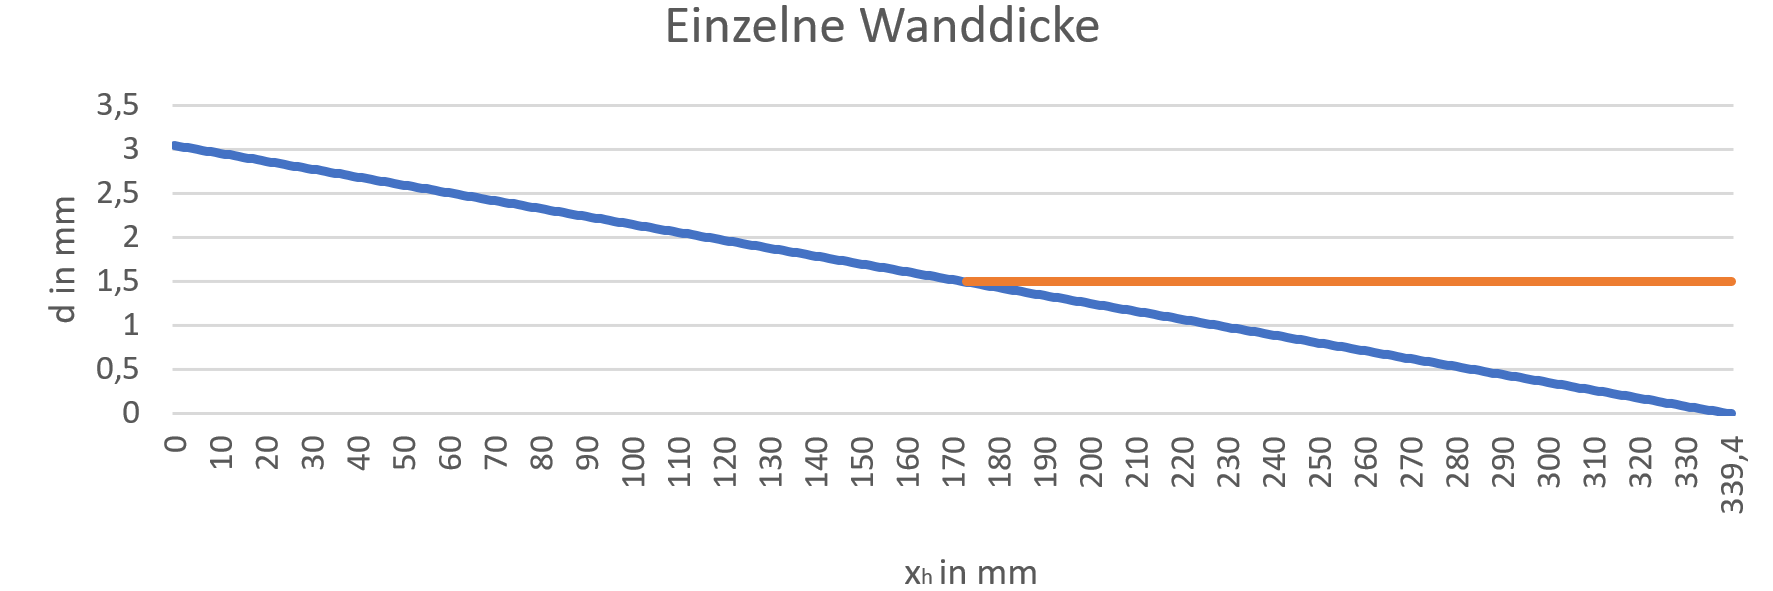
\includegraphics[width=0.85\textwidth]{d_einzel.png}
	\caption{Der Verlauf der Wanddicke $d$ in Abhängigkeit vom Abstand zur Einspannung}
	\label{abb_d_einzel}
\end{figure}\\
Nun steht schon mal eine erste Geometrie des Grid Fins, jedoch benötigen auch die zusätzlichen Designelemente, die aus dem morphologischen Kasten gewählt wurden, eine Festlegung ihrer genauen Werte. Einer davon ist der Pfeilungswinkel $\Lambda_\mathrm{lokal}$, der in Abbildung \ref{abb_lok_Tal} und \ref{abb_lok_Berg} dargstellt ist.
\begin{figure}[h]
	\begin{minipage}[t]{0.45\linewidth}
		\centering
		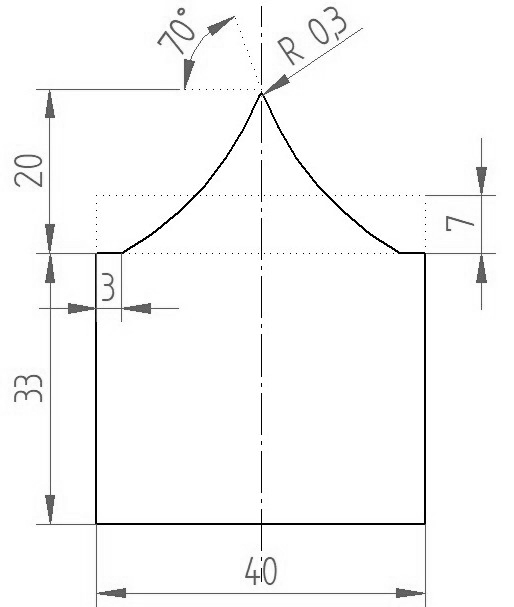
\includegraphics[width=0.9\textwidth]{Pfeil_lok.png}
		\caption{Die geometrischer Zusammenhängen einer gepfeilten Zellwand im Tal-Typus}
		\label{abb_lok_Tal}
	\end{minipage}
	\hfill
	\begin{minipage}[t]{0.45\linewidth}
		\centering
		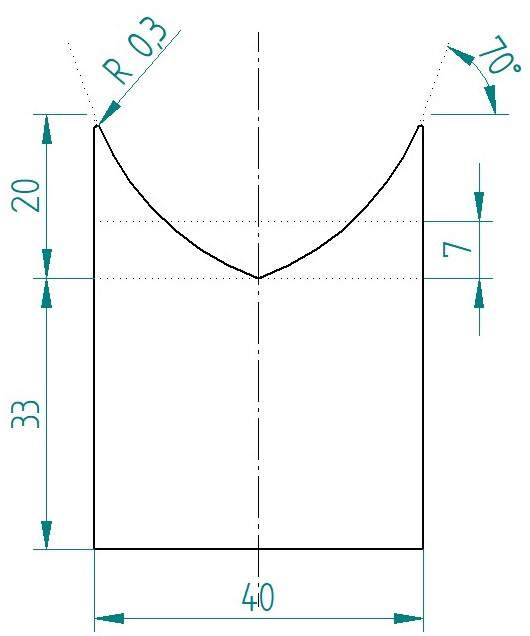
\includegraphics[width=0.9\textwidth]{Pfeil_lok2.png}
		\caption{Die geometrischen Zusammenhänge einer gepfeilten Zellwand im Berg-Typus}
		\label{abb_lok_Berg}
	\end{minipage}
\end{figure}\\
Je größer dieser ist, desto geringer ist die axiale Kraft, doch große Pfeilung schwächt gleichzeitig die Sehne in den Tälern. Als Kompromiss wird der Pfeilungswinkel an den \textbf{Spitzen} zu $\mathbf{\Lambda_\mathrm{lokal}=70^\circ}$ mit einer Abrundung von $0,3$ mm definiert, während zu den Tälern hin ein Tangentenbogen die Neigung abflachen lässt. Die $70^\circ$ entsprechen einem Machkegel bei $Ma = 3.0$, was ungefähr der Zustand ist, bei dem im normalen Missionsablauf die höchsten Kräfte auftreten. Eine stärkere Pfeilung würde das Verhalten bei noch höheren Machzahlen verbessern, jedoch auch zu einer stärkeren Schwächung im Bezug auf thermische und mechanische Belastung führen. Der Berg soll $20$ mm höher liegen als das Tal und die äußeren $3$ mm im Tal werden für den Tal-Typus flach modelliert, sodass in den Schnittpunkten der Zellwände diese immer auf der gleichen Höhe aufeinandertreffen. Für den Berg-Typus ist dies nicht nötig, sodass hier die Tangentenbögen im Tal direkt aufeinander treffen. Die Fläche dieser Pfeilung entspricht einem Rechteck gleicher Breite mit der Höhe $7$ mm. Um also auf eine gemittelte Sehnenlänge von $s=40$ mm zu kommen, muss sich noch $33$ mm restliche Wand unter der Pfeilung befinden.
Auch der Wandquerschnitt soll sich zuspitzen und der zugehörige Winkel wird für das Gitter ebenso entsprechend Abbildung \ref{abb_wandq} auf $70^\circ$ gesetzt. 
\begin{figure}
	\centering
	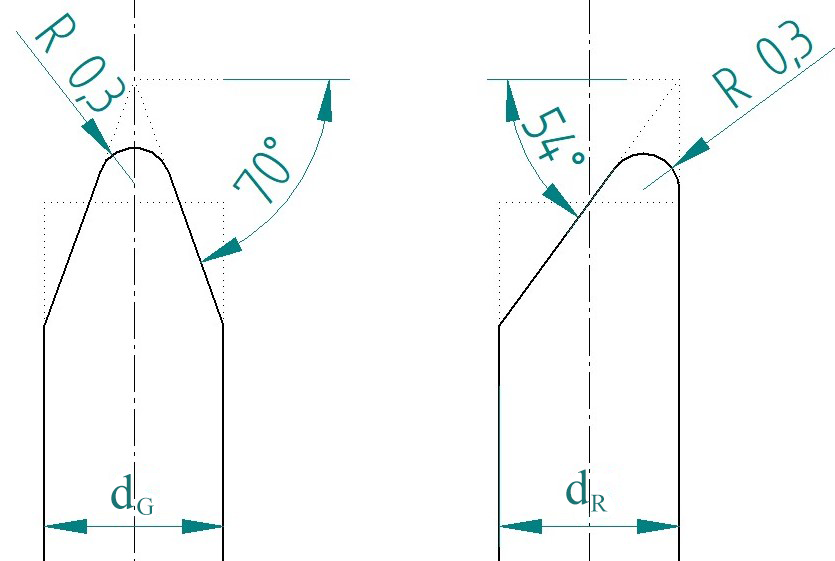
\includegraphics[width=0.5\textwidth]{Wandquerschnitt.png}
	\caption{Zuspitzung der Wände im Querschnitt}
	\label{abb_wandq}
\end{figure}\\
Die Position ist wieder so gewählt, dass die gemittelte Sehnenlänge sich immer auf dem Wert befindet, der durch die lokale Pfeilung vor Ort herrschen soll. Die Rahmenwände haben nur auf einer Seite eine Schräge. Der Winkel wurde hier auf\ $54^\circ$ herabgesetzt, sodass Rahmen und Gitter bei gleicher Wandstärke und Sehnenlänge dieselbe maximale Höhe haben.

Die Krümmung soll für die Vorderkante der gemittelten Sehne ausgelegt werden, also für den Fall, dass keine Pfeilung oder Zuspitzung vorliegt (gepunktete Linie). Da an den Bergen der Pfeilung die Spitze $13$ mm und mit der Zuspitzung bei eine Wandstärke von $4$ mm einen weiteren Millimeter über der nominelle Sehne liegt, müssen noch mindestens $14$ mm auf die $550$ mm Raketenradius addiert werden. Somit wird der \textbf{Krümmungsradius} auf $\mathbf{570}$ \textbf{mm} gesetzt, sodass im eingeklappten Zustand ein $6$ mm breiter Spalt zwischen Rakete und Grid Fin bleibt. Dieser stellt sich, dass weder durch Vibrationen beim Start oder auf Grund von thermischer Ausdehnung die Spitzen gegen den Rumpf stoßen und ihn oder sich selbst beschädigen.
\\~\\
Es sind noch weitere Optionen möglich, mit denen sich die Grid Fins modifizieren lassen würden. Diese werden hier jedoch zunächst nur kurz vorgestellt und erst nach den ersten Analysen beurteilt, ob sie eventuell doch noch implementiert werden sollen.

Die additive Fertigung des Grid Fins ermöglicht neue Optionen, die für klassische Herstellungsverfahren nicht wirtschaftlich umsetzbar sind. So können zum Beispiel Kanäle in das Material integriert werden, welche genutzt werden können, um den Werkstoff zu kühlen oder gar das Air Flush Data System (FADS) mit weiteren Drucksensoren ergänzen. Es wäre auch denkbar, diese einfach nur zur weiteren Gewichtsreduzierung zu nutzen.

Es könnten auch die scharfen Kanten, die senkrecht zur Strömung liegen, abgerundet werden, um so einen besseren Kraftfluss zu erlauben.
\\~\\
Zum Schluss muss an dieser Stelle noch angemerkt werden, dass 3D-Drucker natürlich nur eine begrenzte Auflösung haben. Je nach Hersteller kann somit die minimale Wandstärke $0,4-1,0$mm \cite{eos, preise} und die Schichtdicke $0,04-0,075$mm \cite{preise} betragen. Die Ausrichtung im Drucker hat also auch Einfluss auf den Detailgrad. Somit kann es sein, dass die spitzen Kanten und die Pfeilung in der Fertigung stumpfer werden, als sie ausgelegt wurden. Auch das Hinzufügen von Kanälen ist nur möglich, wenn die Wände dick genug sind.
\subsection{Modellierung in CAD}
Da das Design nun feststeht, soll es auch in einem CAD-Programm modelliert werden. Hier wird Solid Edge der Siemens PLM Software Inc. verwendet. Zunächst wird der Grundriss des Grid Fins (vgl. Abbildung \ref{abb_grundriss}) mit den soeben festgelegten Maßen extrudiert. Dieses Volumen wird beidseitig jeweils konkav oder konvex durch Zylinder mit dem Radius $570$ mm begrenzt, deren Symmetrieachsen um $33$ mm versetzt sind, um zunächst eine Sehne von eben dieser Länge zu erzeugen.
\begin{figure}[h]
	\centering
	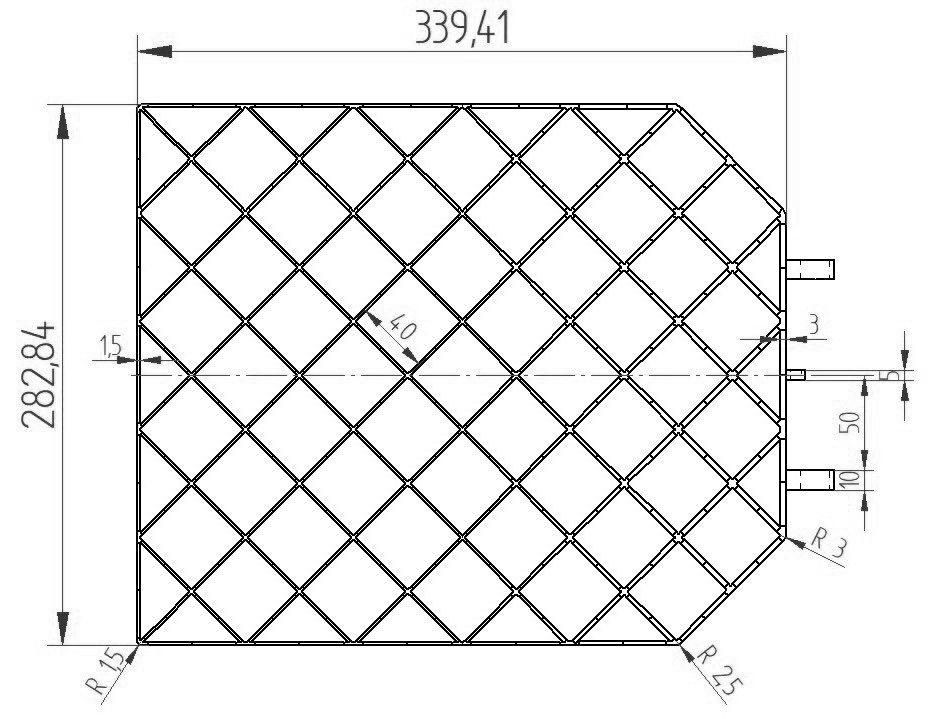
\includegraphics[width=0.6\textwidth]{grundriss.jpg}
	\caption{Grundriss des Grid Fins}
	\label{abb_grundriss}
\end{figure}
\begin{figure}[h]
\centering
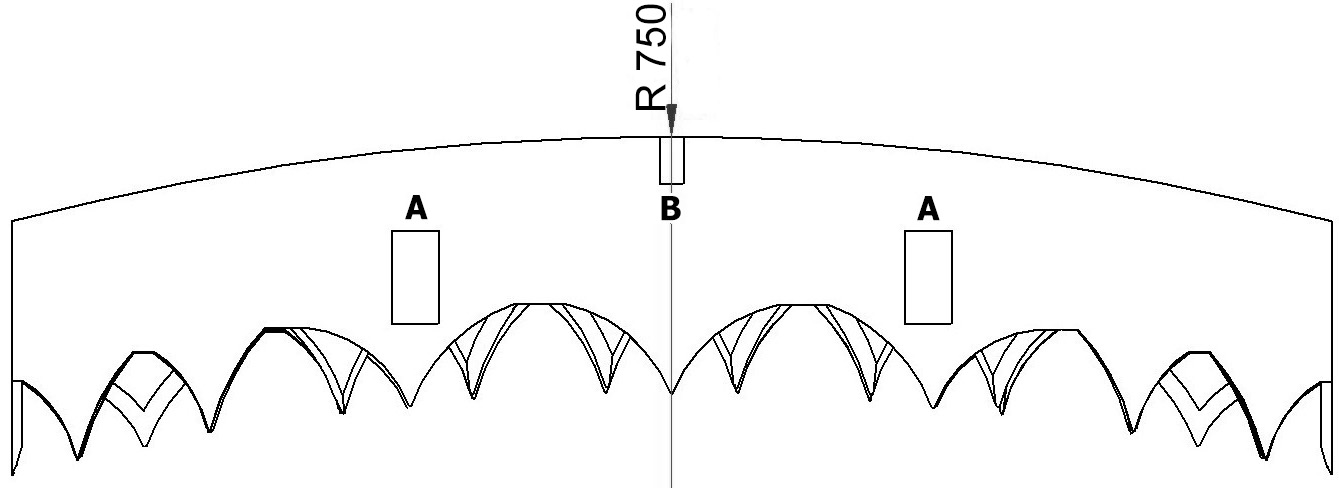
\includegraphics[width=0.5\textwidth]{koerper.jpg}
\caption{Krümmung des Grid Fins}
\label{abb_körper}
\end{figure}\\
Anschließend wird eine Halterung zur Befestigung und Bewegung der Grid Fins modelliert. Diese setzt sich aus der Halterung A, um die sich der Grid Fin beim Ein- und Ausklappen dreht, und Halterung B, an der die Kraft, die diese Bewegung bewirkt, angreift, zusammen. Sie sind entsprechend Abbildung \ref{abb_grundriss} und \ref{abb_halterung} von der Mittellinie und dem untersten Punkt auf Höhe der Mittellinie aus definiert.
\begin{figure}[h]
	\centering
	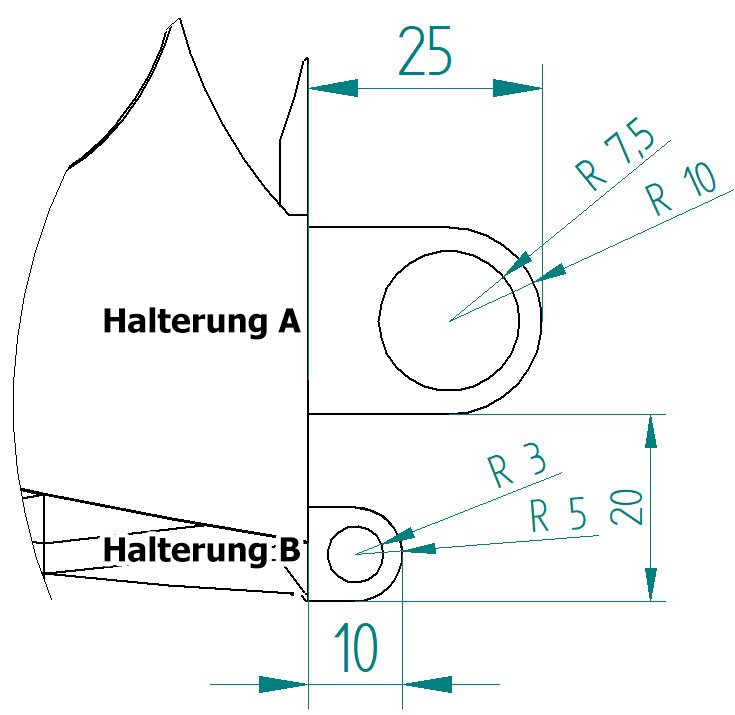
\includegraphics[width=0.35\textwidth]{Halterung.png}
	\caption{Einspannung am Grid Fin}
	\label{abb_halterung}
\end{figure}\\
Als nächstes wird auf der konkaven Seite die lokale Pfeilung nach Abbildung \ref{abb_lok_Tal} und \ref{abb_lok_Berg} hinzugefügt. Da diese Seite des Grid Fins jedoch nicht gerade sondern krumm ist, weicht die Realität leicht von diesen Abbildungen ab. Die Position der Täler und Berge orientiert sich zwar an der Höhe der Kante an der jeweiligen Position, aber $20$mm der Berge gehen weiterhin in die Richtung, aus der später die Anströmung kommen wird, und die flachen Segmente beim Tal-Typus bleiben senkrecht zu dieser Richtung, anstatt sich an der Tangentenebene des Zylindermantels zu orientieren. Auch die Breite dieser Pfeilungssegmente von $40$mm durch die Krümmung minimal ab. Des Weiteren beträgt eben diese Breite bei den meisten Rahmenwänden das $\sqrt{2}$-fache, da sie die Zellen in ihrer Diagonalen teilen. Die restlichen Bedingungen bleiben jedoch, sodass weiterhin an der Spitze ein Winkel von $\Lambda_{lokal} = 70^\circ$ herrscht und nur die Tangentenbögen weiter gehen.

Zuletzt wird der Wandquerschnitt sowohl auf der konkaven also auch der konvexen Seite angepasst, indem Fasen des entsprechenden Winkels zu einer Zuspitzung führen, die anschließend abgerundet werden.
\\~\\
Somit hat nun der das erste Modell seine gewünschte Gestalt angenommen, sodass im Anschluss die entsprechende Aktuatorik entworfen werden kann. Im nächsten Kapitel werden dann ausgehend von diesem CAD-Modell Analysen dürchgeführt, anhand derer Optimierungen erfolgen.
\section{Komponentenrecherche und -auswahl der Aktuatorik}
Als Nächstes werden nun die Ergebnisse der Komponentenrecherche beschrieben und auf Grund der Systemanforderungen mit Hilfe der morphologischen Kästen -soweit dies möglich ist- eine vorläufige Wahl getroffen.
\subsection{Peripherie}
Für alle der drei Energiemedien sind schon Vertreter in der Rakete installiert, die unter Umständen genutzt werden könnten. Da sich die Grid Fin Aktuatorik im demselben Abschnitt wie die Bordelektronik der ersten Stufe befindet, ist hier auch schon eine Leitung zu den Batterien gelegt, mit deren Hilfe Elektromotoren betrieben werden können. So wird mit ihnen zum Beispiel auch die elektrischen Treibstoffpumpen für die Triebwerke mit Strom versorgt. Somit liegt direkt auch schon ein Hochdruckfluid vor, welches als Druckmittel für die Hydraulik genutzt werden könnte. Da sich dieses jedoch am anderen Ende der Rakete befindet und dafür sowohl ein Eingriff in die komplexen Triebwerke als auch eine Abhängigkeit von vorhandenem Treibstoff zu Stande kommt, ist dies eine weniger plausible Möglichkeit. Deshalb ist eine eigene elektrische Pumpe und eigenes Druckmittel eine realistischere Umsetzung für eine Hydraulik. Für eine Pneumatik könnte jedoch ein vorhandenes System genutzt werden. Der Heliumtank für den Druckausgleich in den Tanks liegt direkt unterhalb der Elektronik und es existieren sogar schon Leitungen, die das Gas in diesen Bereich der Rakete für das RCS transportieren.
\\~\\
Da sowohl für den Klappwinkel als auch den Steuerwinkel unterschiedliche Anforderungen existieren, die auch andere Lösungsmöglichkeiten zulassen, werden diese im Folgenden getrennt betrachtet.
\subsection{Klappwinkel}
Der Klappwinkel muss eine Drehung um $90^\circ$ durchführen. Dies soll durch die lineare Bewegung einer Hubstange realisiert werden. Damit im ausgeklappten Zustand ($\Lambda = 90^\circ$) die Kraft ideal durch die Stange geleitet werden kann, soll sich dann die Halterung B auf der gleichen Höhe wie die Bewegungsachse befinden. Um aus der linearen Bewegung eine Drehung zu erhalten, muss die Hubstange über eine weitere Stange gelenkig mit der Halterung verbunden werden. Mit einer Länge der Verbindungsstange von $43$ mm, können aus den Beziehungen, die in Abbildung \ref{abb_hub} zu sehen sind, der benötigte Hub ermittelt werden.
\begin{figure}[h]
	\centering
	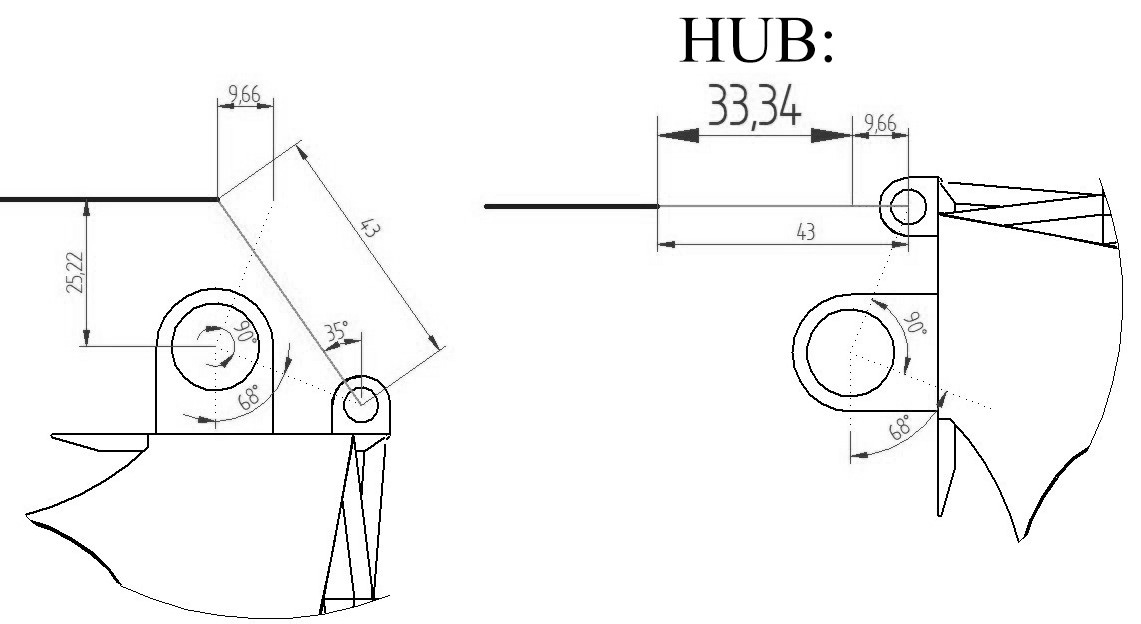
\includegraphics[width=\textwidth]{Hub.jpg}
	\caption{Der Hub des Klappwinkels}
	\label{abb_hub}
\end{figure}\\
Obwohl die wirkenden Kräfte und Momente im Vergleich zur den aerodynamischen relativ gering sind, kommt es während des Wiedereintritts und besonders beim Auslösen des Ballonschirms zu sehr hohen Belastungen. Somit fällt die pneumatische Option weg, da diese nicht die entsprechenden Haltekräfte aufbringen kann. Übrig bleibt dann nur noch eine hydraulische oder elektrische Lösung. Ein hydraulisches System bräuchte zwar auch einen Elektromotor, um die Pumpe zu betreiben, hätte aber den Vorteil, dass eine Pumpen-Motor-Kombination für alle vier Grid Fins gleichzeitig ausreichen würde. Ein hydraulisches System bringt jedoch auch einige Nachteile mit sich. Zum einen würde die Gefahr bestehen, dass bei einem Fehler alle Grid Fins unbrauchbar oder gar missionsgefährdend werden. Im Gegensatz dazu zeichnen sich Systeme, die pro Grid Fin unabhängig voneinander sind, dadurch aus, dass die nicht defekten Grid Fins einen Ausfall eventuell ausgleichen könnten. Zum anderen würde die Lösung voraussichtlich eine merklich höhere Masse wegen des Hydraulikfluids benötigen. Des Weiteren muss sich der Hubzylinder bei einer Veränderung des Steuerwinkels mitbewegen. Dies erhöht wiederum die Anforderungen an die Leitungen und sorgt für mehr Anfälligkeitspotential. Schlussendlich ist der entscheidendste Faktor die hohen Kosten eines solchen hydraulischen Systems. Auch wenn eine elektrische Lösung vier mal gebraucht wird, sorgt die höhere benötigte Leistung und die vielen teuren Bauteile dafür, dass sich die Hydraulik in diesem Anwendungsfall nicht rentiert. Die Turbine müsste noch immer vier mal auftauchen und entspricht preislich ungefähr einem Elektromotor mit gleicher Leistung, sodass die Pumpe und der zugehörige Motor nur extra Kosten verursachen würden. Bei den elektrischen Motoren gibt es nun auch wieder zwei Varianten, zwischen denen sich wählen lässt. Es kann entweder direkt ein Linearmotor verwendetet werden, der direkt den Hub ausführt, oder ein klassisch rotierender Motor, dessen Drehung über ein Spindelgetriebe in eine Linearbewegung umgewandelt wird. Ein Linearmotor wäre zwar die kostengünstigere Option, jedoch ist er deutlich größer und somit auch schwerer, als die Alternative mit Spindelgetriebe. Die größeren Dimensionen des Linearantriebs würden auch ein größeres System für den Steuerwinkel bedeuten, was wiederum zu noch mehr Masse führt und eine höhere Leistungsanforderung an den Steuerwinkelaktuator bewirkt.
\\~\\
Somit wird für die Klappbewegung ein \textbf{rotierender Elektromotor} mit \textbf{Spindelgetriebe} verwendet. Als letztes gilt es noch die Frage der Lagerung zu klären. Da die größten Kräfte erst angreifen, wenn der Klappwinkel nur noch still steht, ist eine reibungsarme Lagerung nicht ganz so wichtig. Dennoch soll es nicht dazu kommen, dass sich der Mechanismus festklemmt und somit ein Ausklappen der Grid Fins verhindert wird. Damit das Spindelgetriebe nicht aus seiner Halterung gehebelt werden kann, muss die Hubstange noch an einer zweiten Stelle aufliegen. Deswegen wird auf die Welle ein \textbf{Linearlager} montiert, durch das die Hubstange geführt wird. Sowohl in die Verbindung von Hubstange zur Verbindungsstange, als auch die Halterungen A und B sollen \textbf{Wälzlager} montiert werden, deren genau Gestalt erst im nächsten Kapitel festgelegt wird, wenn die endgültigen Maße der Halterung berücksichtigt werden können.
Da auch die Wahl der Spindel und des Motors stark von der Geometrie des Grid Fins, insbesondere der Halterung und den damit einhergehenden Hebeln, abhängt, wird an dieser Stelle noch keine getroffen. Erst nachdem im nächsten Kapitel die endgültige Geometrie durch FEM-Analysen und Optimierungen festgelegt wird, kann auch eine genauere Auslegung dieser Aktuatorik stattfinden.
\subsection{Steuerwinkel}
Auch für den Steuerwinkelaktuator können wieder Pneumatik, Hydraulik und Elektrik gegeneinander abgewogen werden. Neben den Argumenten, die schon für den Klappwinkel genannt wurden, kommt für den Steuerwinkel noch die Bewegung unter Last mit vielen Richtungswechsel hinzu. Auch für diesen Anwendungsfall bietet der \textbf{Elektromotor} (natürlich rotierend) die besten Eigenschaften. Ein hydraulisches System würde nur unnötig die Trägheit erhöhen, wo hingegen ein Elektromotor die vielen schnellen Richtungswechsel ideal leisten kann.
Ein entscheidendes Kriterium für die Wahl des Motors ist die Fähigkeit, ein Moment aufzubringen, um den maximalen Ausschlag beim "Max Q"\ zu halten. Natürlich muss das wirklich erreichte Moment etwas höher liegen, sodass dieser Ausschlag in endlicher Zeit erreicht wird.
\begin{equation}\label{eq_M_min}
	M_{Antrieb} > M_m(\delta = 20^\circ) = 89,1\mathrm{ Nm}
\end{equation}
Elektromotoren haben aber üblicher Weise eine Drehzahl, die deutlich über der benötigten Drehrate liegen, sodass ein relativ leistungsschwacher Motor verwendet werden kann. Es besteht dann die Möglichkeit, das Moment über ein Getriebe auf Kosten der Drehzahl zu erhöhen. Somit kann ein günstigerer und leichterer Motor verwendet werden, dessen Arbeitsbereich auch deutlich besser ausgenutzt wird. Die große Differenz zwischen den Momenten und Drehzahlen, die ein Motor liefert, und denen, die benötigt werden, verlangt eine hohe Übersetzung. Die einfachste und platzsparenste Möglichkeit bieten hier ein \textbf{Planetengetriebe}. Je größer die Übersetzung ist, desto kleinere und leistungsschwächere Motoren können verwendet werden. Der Motor wird dadurch zwar immer günstiger, die Getriebekosten steigen jedoch. Neben zu geringen Drehzahlen beschränkt auch die Bedingung aus Gleichung \ref{eq_M_min} das Übersetzungsverhältnis nach oben hin. In Hinblick auf Kosten ergibt sich eine Übersetzung von 200 als guter Wert, bei dem die in Frage kommenden Motoren noch immer die notwendige Leistung liefern sollte. Ob dies wirklich der Fall ist, wird in nächsten Kapitel überprüft und hier zunächst nur eine vorläufige Wahl getroffen.

Der Grid Fin soll an dem einen Ende einer Welle mittels einer Gabel so angebracht werden, dass der Mittelpunkt des Gitters genau auf der Achse liegt, nur so sind die geringen aerodynamischen Momente gewährleistet. Im Gegensatz zum Klappwinkel ist hier eine reibungsarme Lagerung sehr wichtig. Auch die statische Bestimmtheit muss gegeben sein, da Kräfte und Momente in alle Richtungen auftreten können. Deswegen werden \textbf{Kegelrollenlager} in O-Stellung verwendet, was eine hohe Steifigkeit bietet. Auf der Seite des Grid Fins stützt sich das Lager gegen eine Wellenschulter, während das Lager auf der anderen durch eine Nutmutter gesichert wird.
Somit ist ein erstes Konzept wie es in Abbildung \ref{abb_Welle} dargestellt ist so weit es geht definiert. Für eine weitere Spezifikation und Optimierung werden die Ergebnisse der im Folgenden stattfindenden Simulationen benötigt.
\begin{figure}[h]
	\centering
	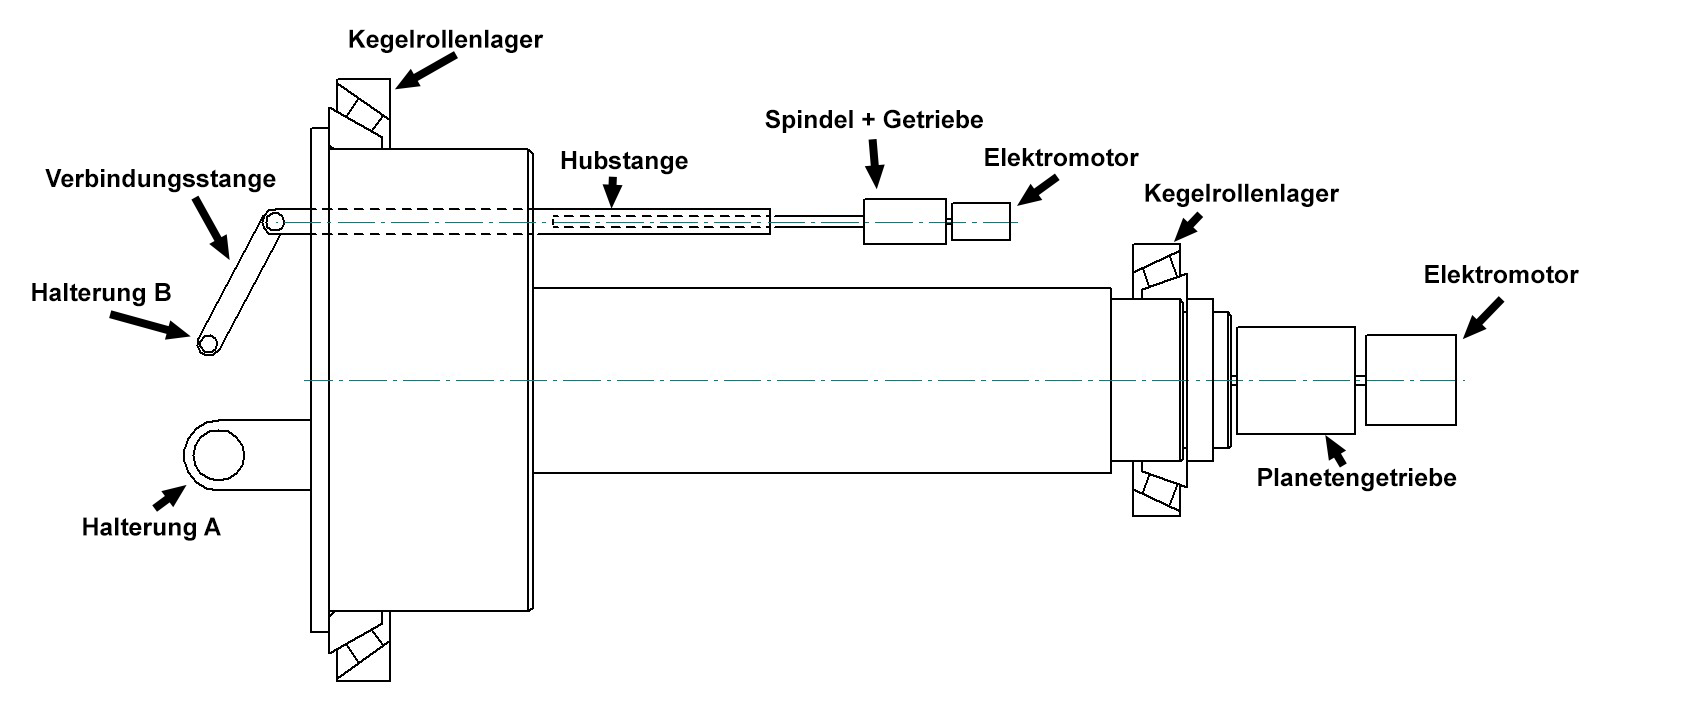
\includegraphics[width=\textwidth]{Skizze Welle.png}
	\caption{Aufbau der Aktuatorik}
	\label{abb_Welle}
\end{figure}\\
